\chapter{Implementación}

% 3: requisitos
% 4: diseño del sistema. arq, back, front, abstracto, estructura general\
% 5: implementacion. especifico

En este capítulo se detalla la implementación de la plataforma desarrollada, describiendo las decisiones técnicas, herramientas y metodologías empleadas para materializar los objetivos planteados. La arquitectura del sistema se fundamenta en la separación clara entre el backend, responsable del procesamiento de datos y la lógica principal de la aplicación, y el frontend, encargado de la presentación e interacción con el usuario. Esta aproximación modular facilita el mantenimiento, escalabilidad y futuras extensiones del sistema. 

\begin{figure}[H]
  \centering
  \fbox{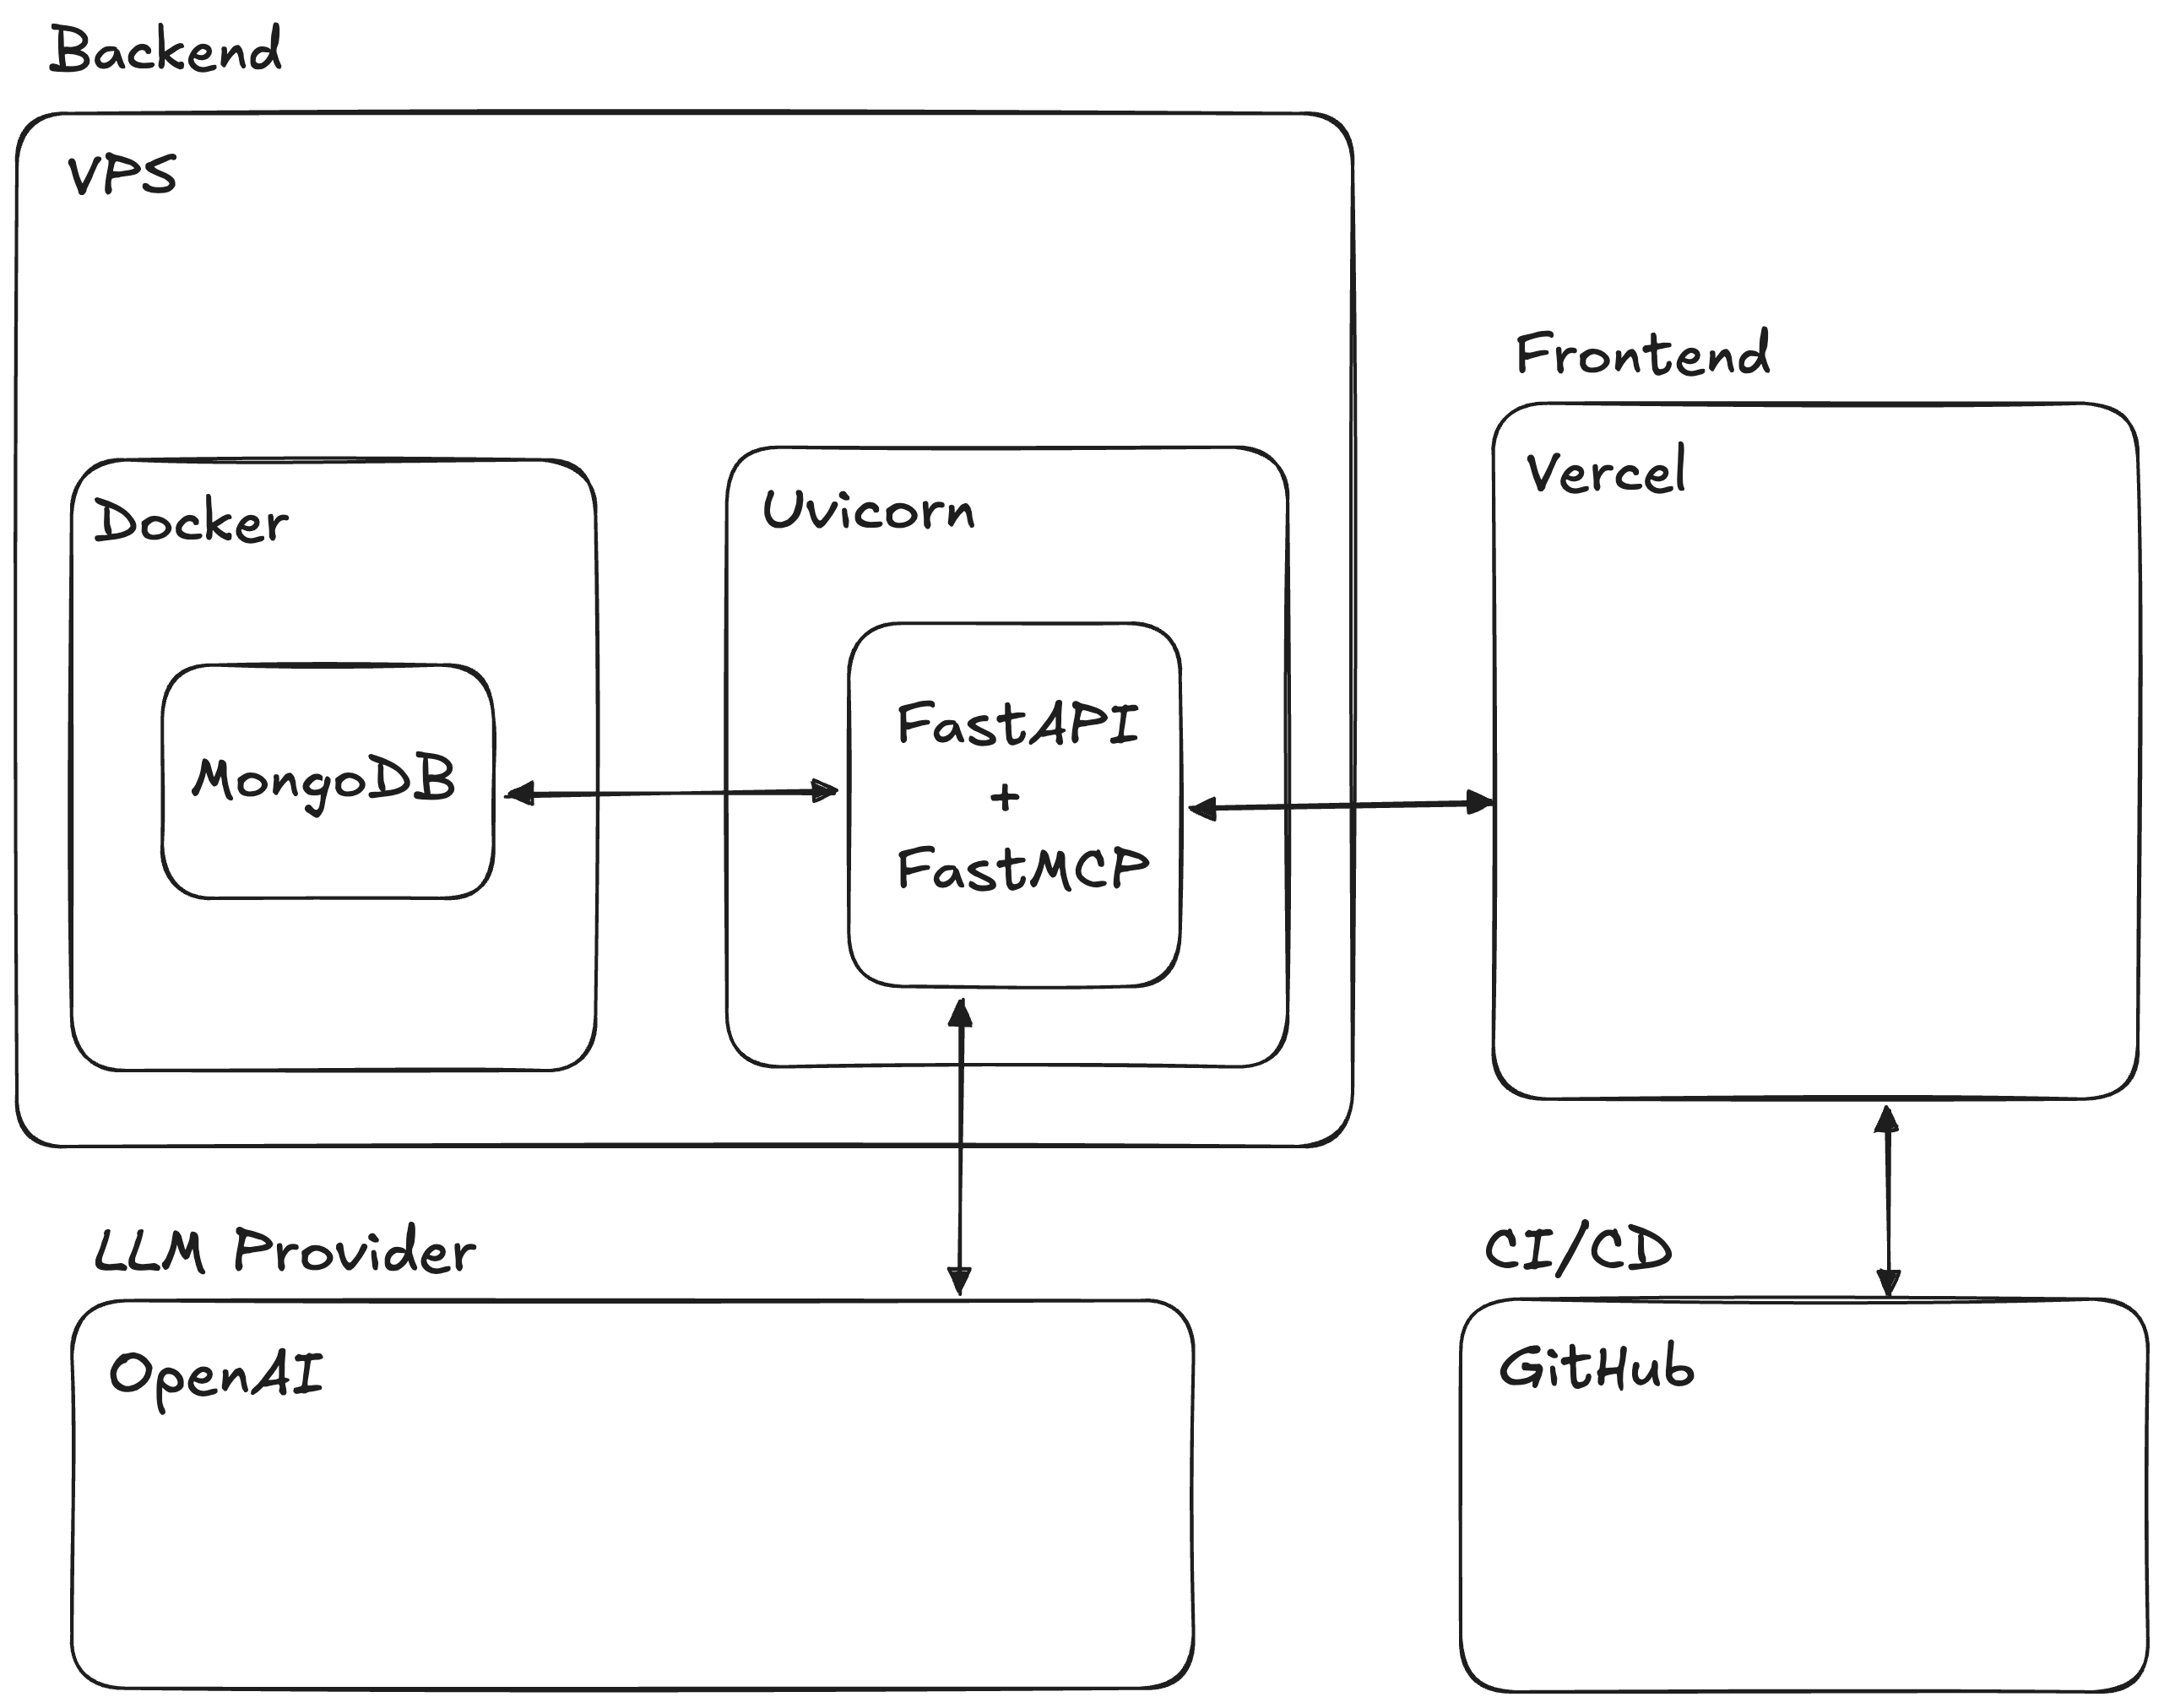
\includegraphics[width=0.9\textwidth]{imagenes/arch1.png}}
  %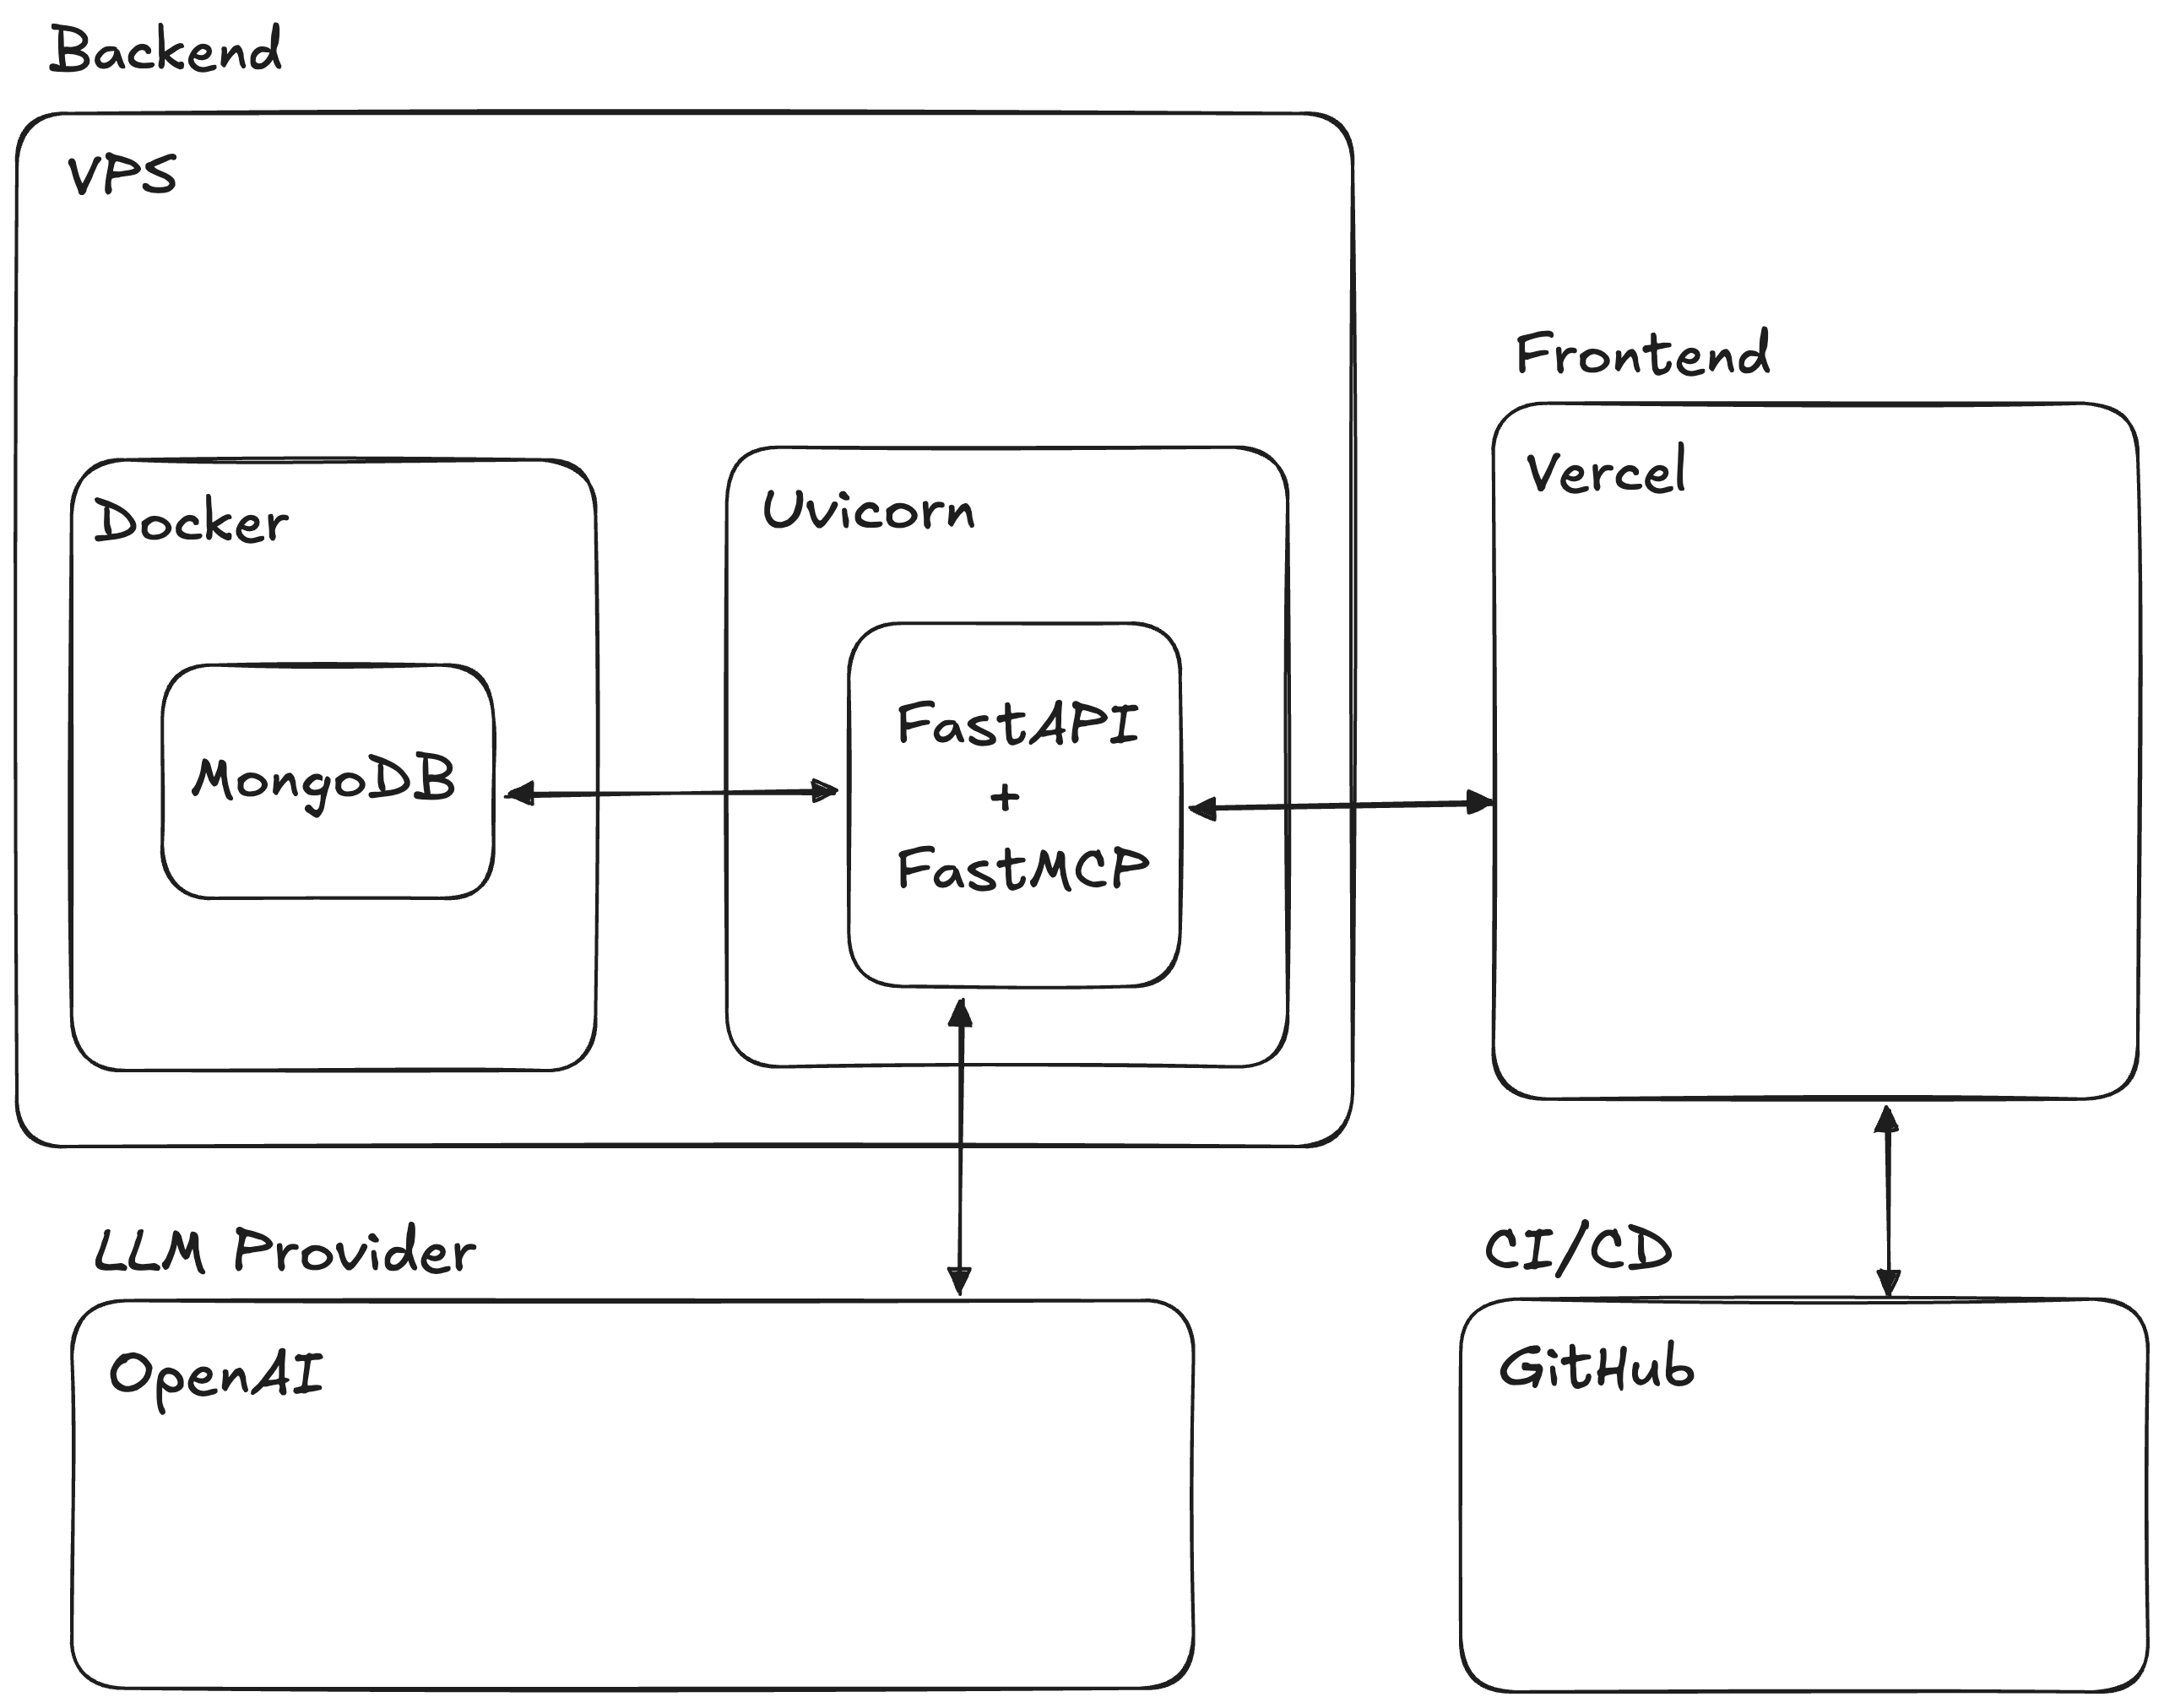
\includegraphics[width=0.9\textwidth]{imagenes/arch1.png}
  \caption{Arquitectura de la aplicación}
  \label{fig:arch1}
\end{figure}

\section{Backend}

El backend constituye el núcleo de la lógica de este trabajo. Se puede dividir en dos elementos: la base de datos MIMIC-IV almacenada en MongoDB con Docker, y la API RESTful con FastAPI que consulta datos, los procesa y los devuelve al cliente. También se encarga de llamar a los LLMs y a ejecutar el servidor MCP. Todo se aloja en un servidor personal y se accede por HTTPS gracias a Cloudflare Tunnels. A continuación profundizamos en esta parte del proyecto.

%\subsection{Almacenamiento de MIMIC-IV en MongoDB}
\subsection{Base de Datos}


Una de las tareas técnicas fundamentales del proyecto ha sido la migración del conjunto de datos, desde su formato original en archivos CSV comprimidos a una base de datos MongoDB. A continuación se explica todo el proceso.


\subsubsection{Desplegando MongoDB}

Para el despliegue de MongoDB se utilizan dos contenedores Docker, en distintos puertos, uno para la versión completa del conjunto de datos, y otro para la versión demo, facilitando así la realización de pruebas sin tener que lidiar con los cientos de millones de datos de la versión completa. Como apoyo al desarrollo, y también en forma de contenedores, se despliegan las herramientas de interfaz gráfica: Portainer para Docker \cite{portainer_ce} y Mongo Express para las bases de datos \cite{mongo_express}. 


\begin{figure}[H]
  \centering
  \fbox{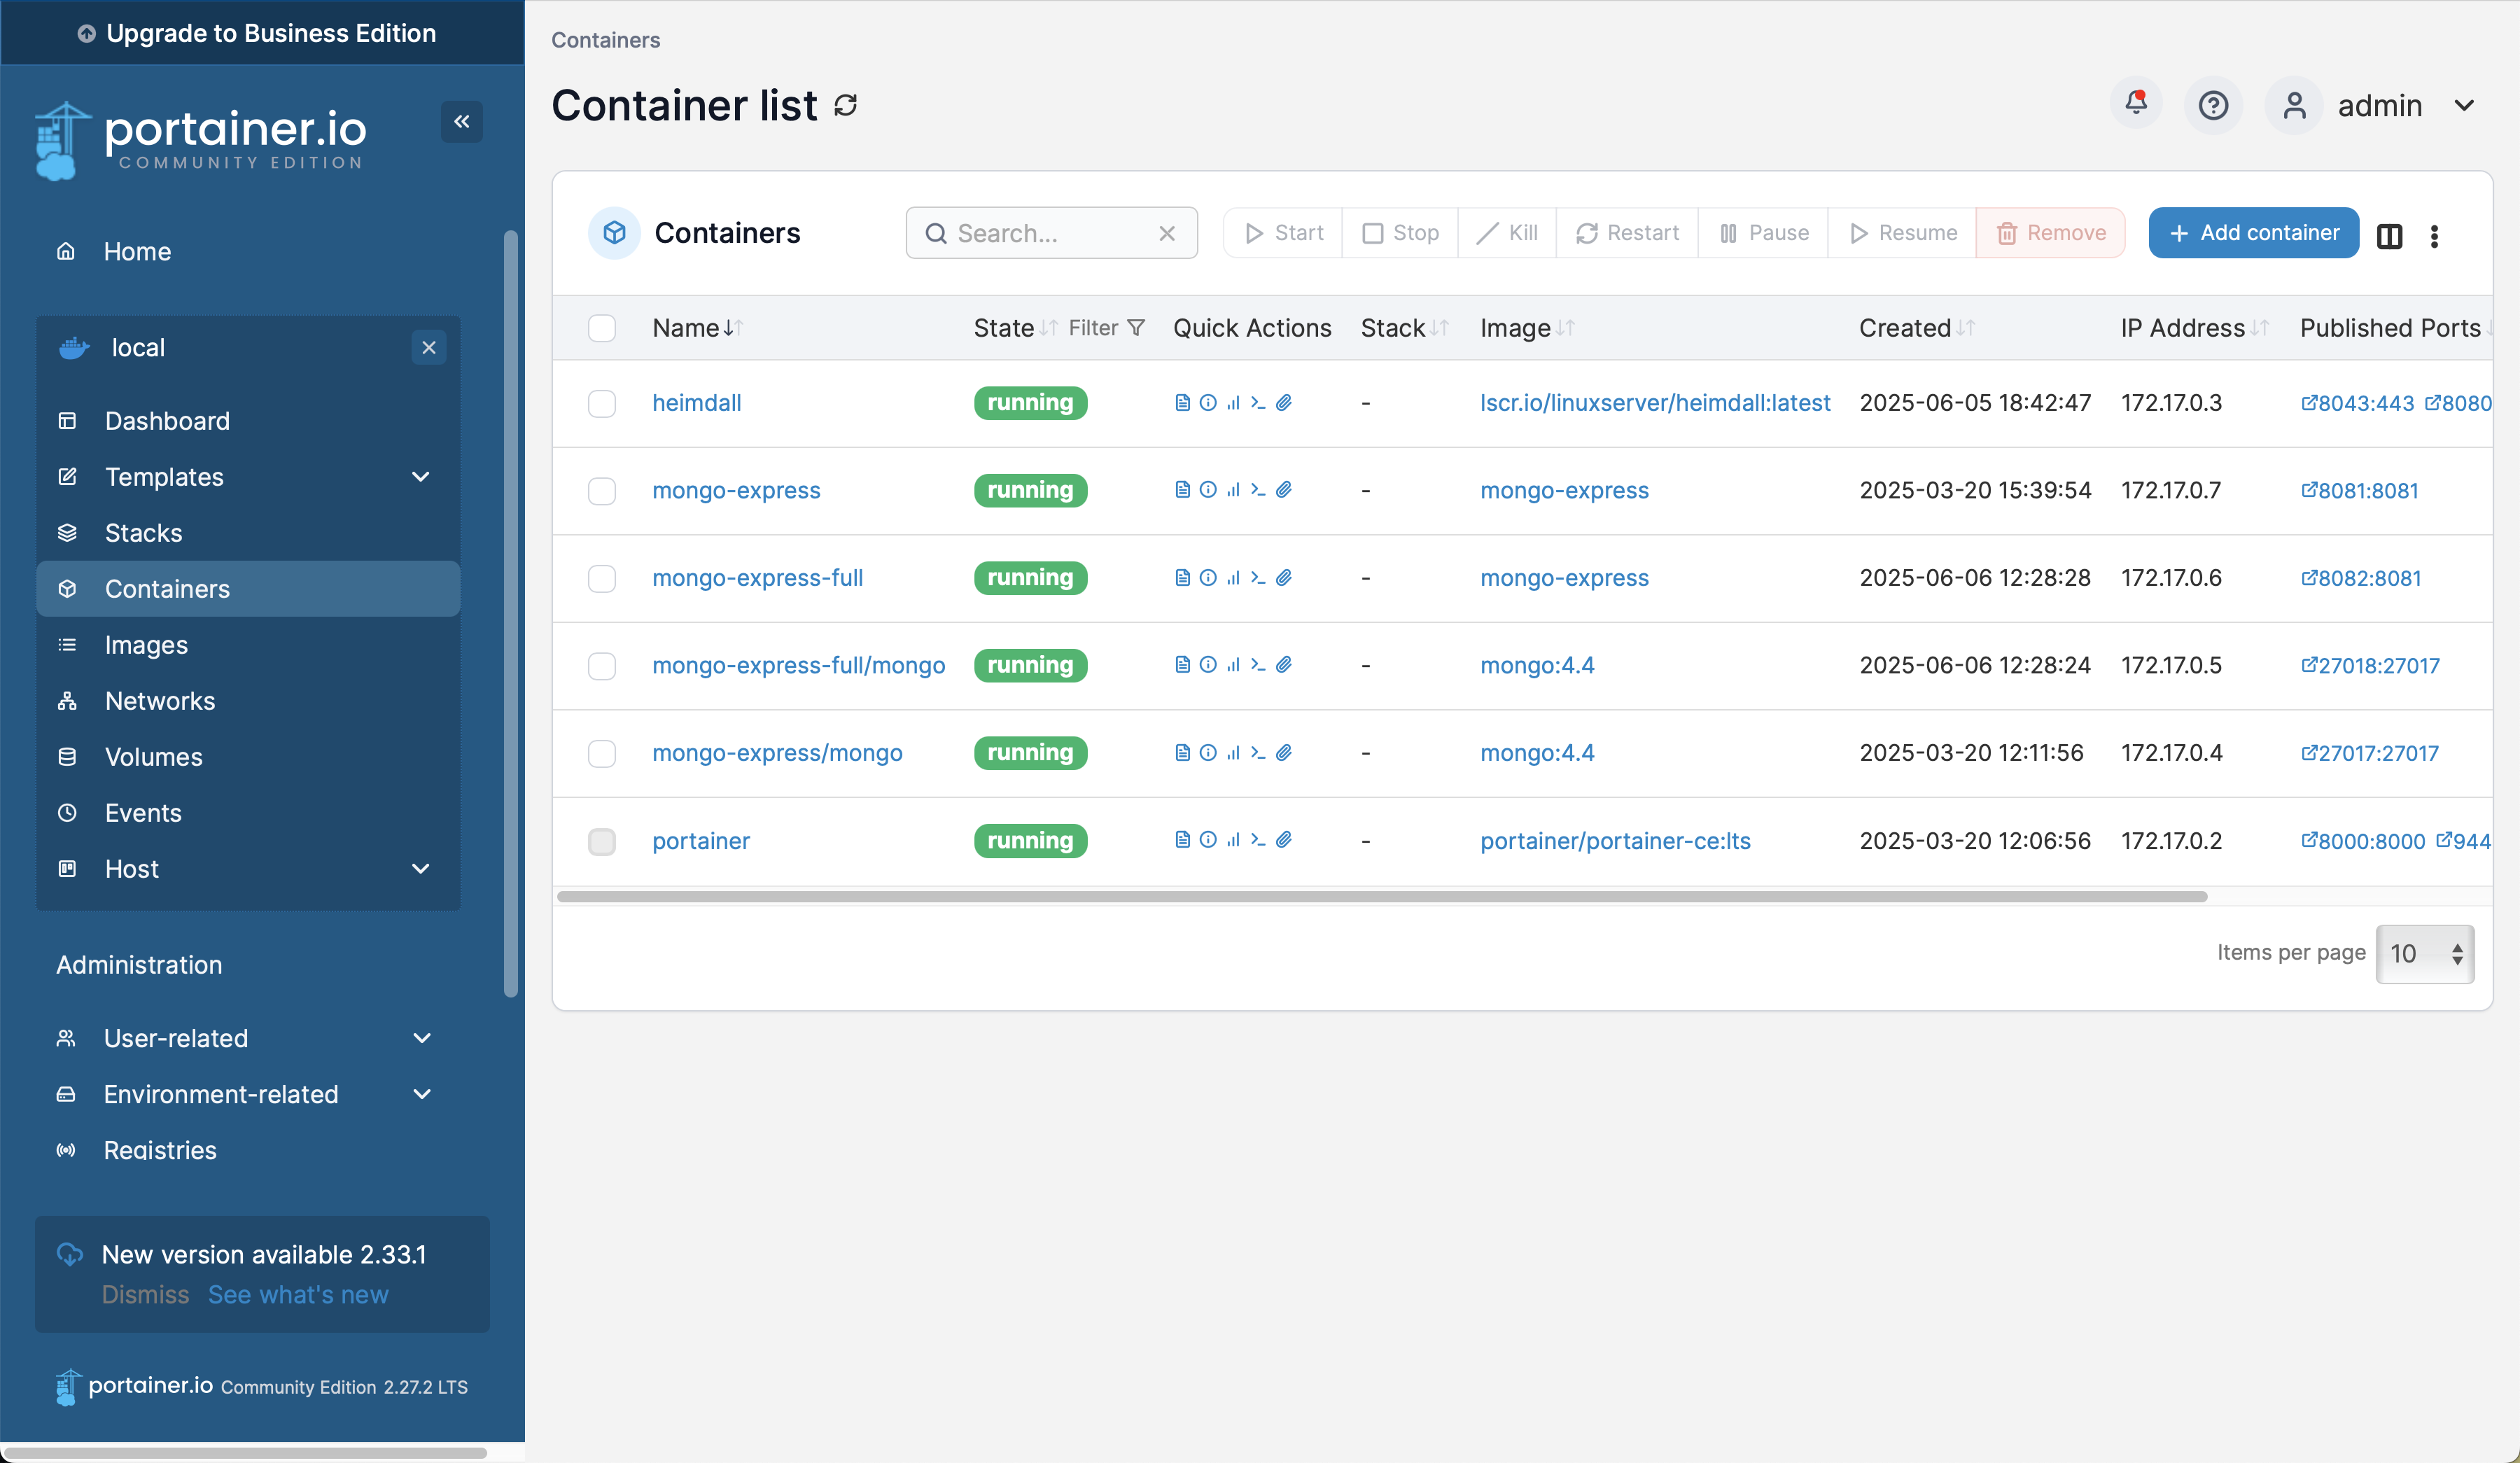
\includegraphics[width=1\textwidth]{imagenes/screenshot3.png}}
  %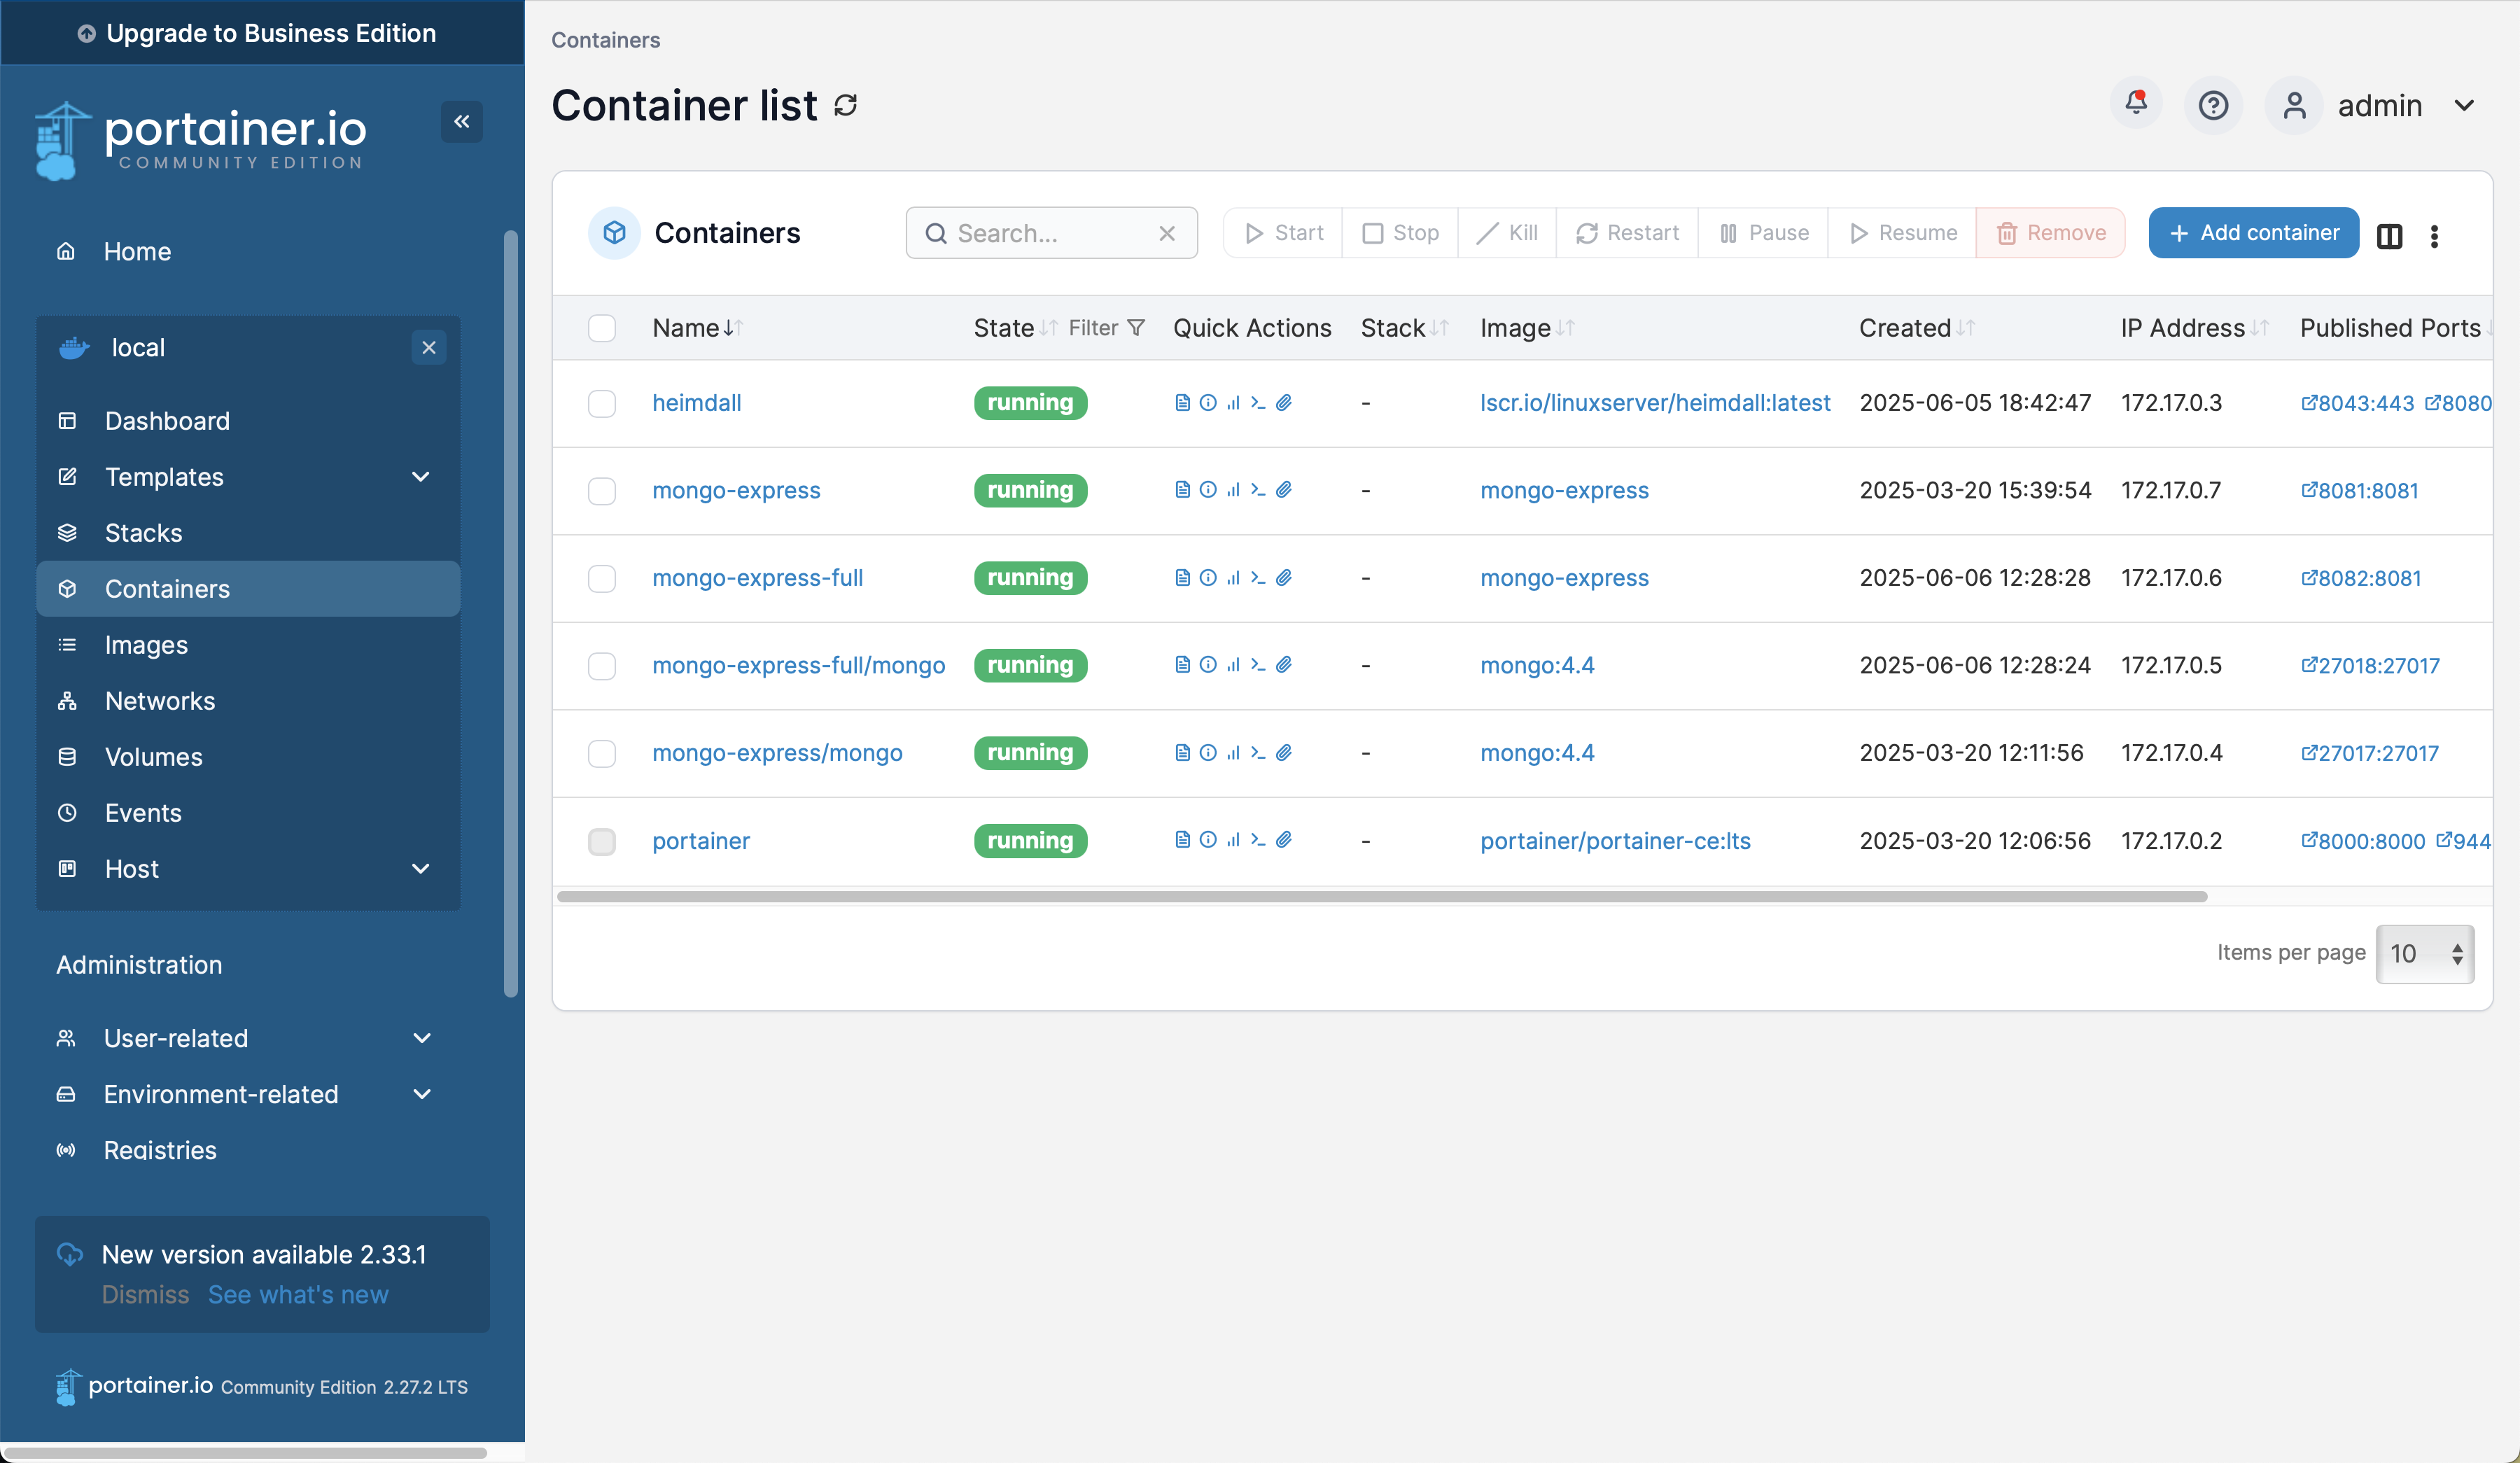
\includegraphics[width=1\textwidth]{imagenes/screenshot3.png}
  \caption{Captura de pantalla de Portainer}
  \label{fig:screenshot3}
\end{figure}


% --------------------
\subsubsection{El proceso de migración}

Se realizó mediante scripts de Python utilizando la librería \texttt{pandas} para la lectura de archivos CSV y \texttt{pymongo} para la inserción en MongoDB. Cada fila del CSV se convierte en un archivo JSON/BSON \cite{mongojsonbson} en MongoDB, donde cada columna es un campo del documento, y cada archivo CSV completo acaba siendo una colección de documentos. Podemos entenderlo mejor, pensando que cada archivo CSV es equivalente a una tabla de una base de datos relacional, y observando la siguiente figura \ref{fig:equivalenciasql}.

\begin{figure}[H]
  \centering
  \fbox{\includegraphics[width=0.8\textwidth]{imagenes/mongodb-vs-sql-1.png}}
  %\includegraphics[width=0.8\textwidth]{imagenes/mongodb-vs-sql-1.png}
  \caption{Equivalencia entre conceptos SQL y NoSQL \cite{equisqlfoto}}
  \label{fig:equivalenciasql}
\end{figure}

Los nombres de las colecciones recibieron el formato \texttt{\textless módulo\textgreater\_\textless tabla\textgreater}. Por ejemplo: \texttt{hosp\_patients}, \texttt{icu\_procedureevents}, etc.

\begin{figure}[H]
  \centering
  \fbox{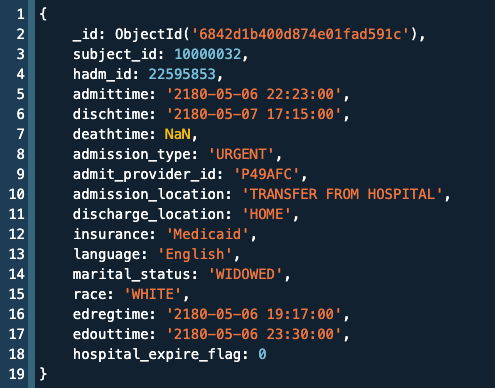
\includegraphics[width=0.6\textwidth]{imagenes/ej_admission.png}}
  %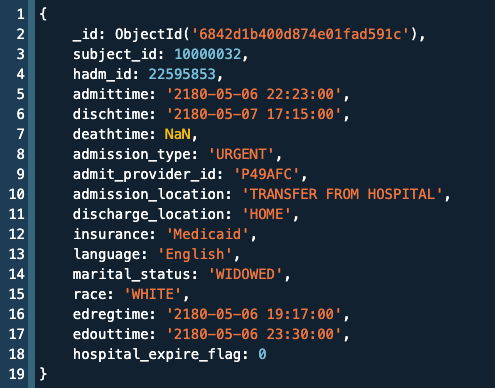
\includegraphics[width=0.6\textwidth]{imagenes/ej_admission.png}
  \caption{Ejemplo de un documento de \texttt{hosp\_admissions}}
  \label{fig:screenshot3}
\end{figure}

Una vez entendida la estructura de los datos de MIMIC-IV, la equivalencia de los archivos CSV a documentos y colecciones de MongoDB, la base de datos ejecutandose con Docker y los scripts preparados, era momento de realizar la migración. 

Todo este proceso se realizó dos veces, para dos versiones distintas de MIMIC-IV: la versión completa, cuyo acceso está restringido y contiene múltiples GBs de información, y la versión demo, que es un subset de 100 pacientes y es de acceso libre \cite{MIMICIV_Demo}. Para la versión completa, el procesamiento se tuvo que realizar por chuncks para evitar el desbordamiento de memoria, que fue un problema recurrente debido a la cantidad masiva de datos.

\begin{figure}[H]
    \centering
    \fbox{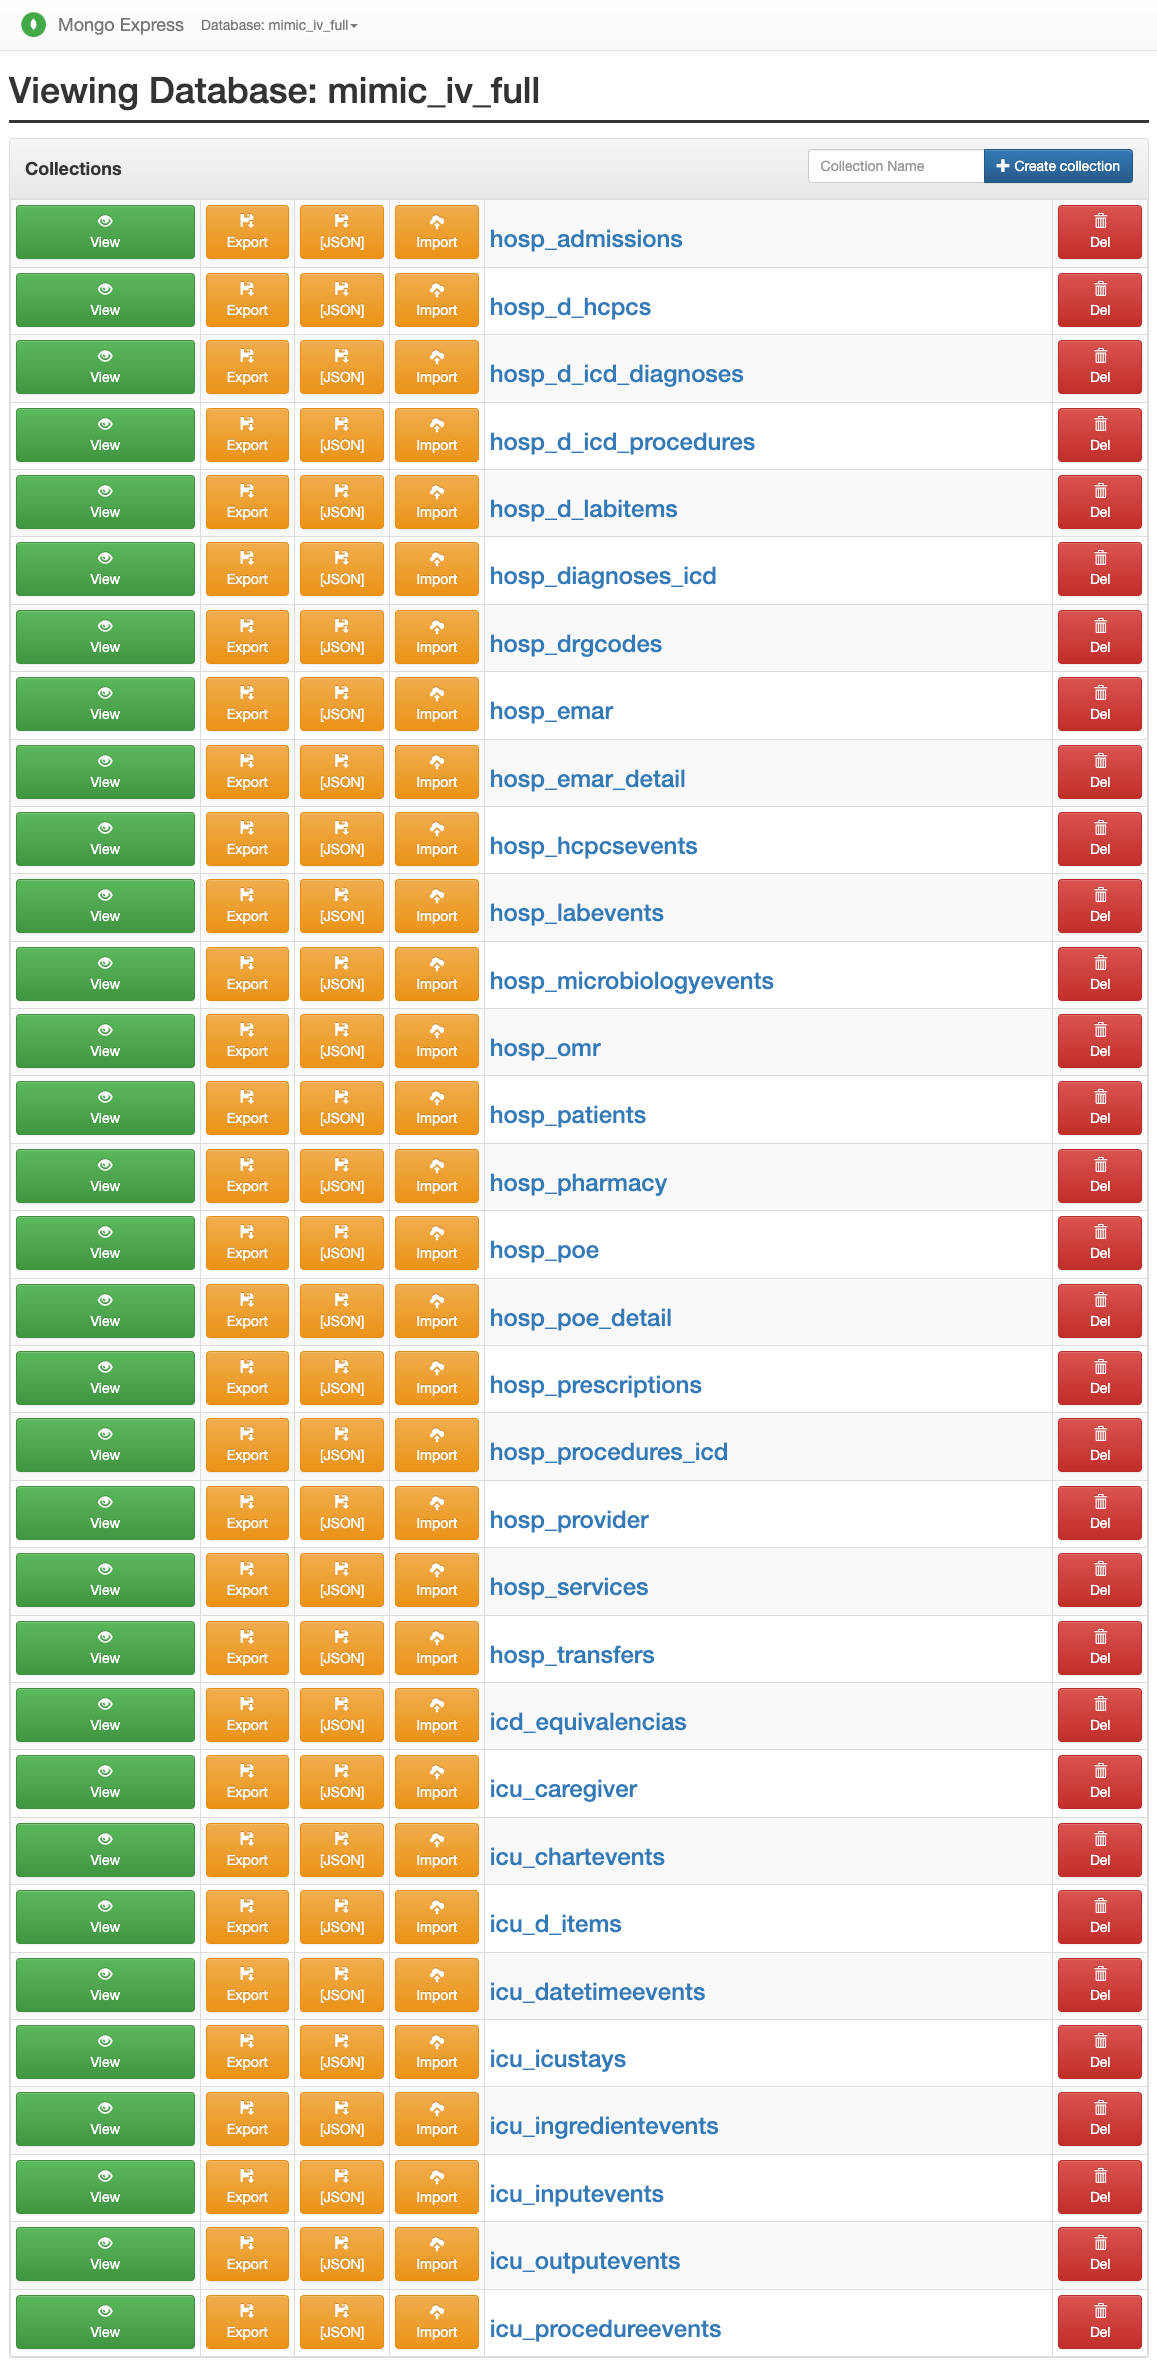
\includegraphics[width=0.8\textwidth]{imagenes/db_full_list.png}}
    %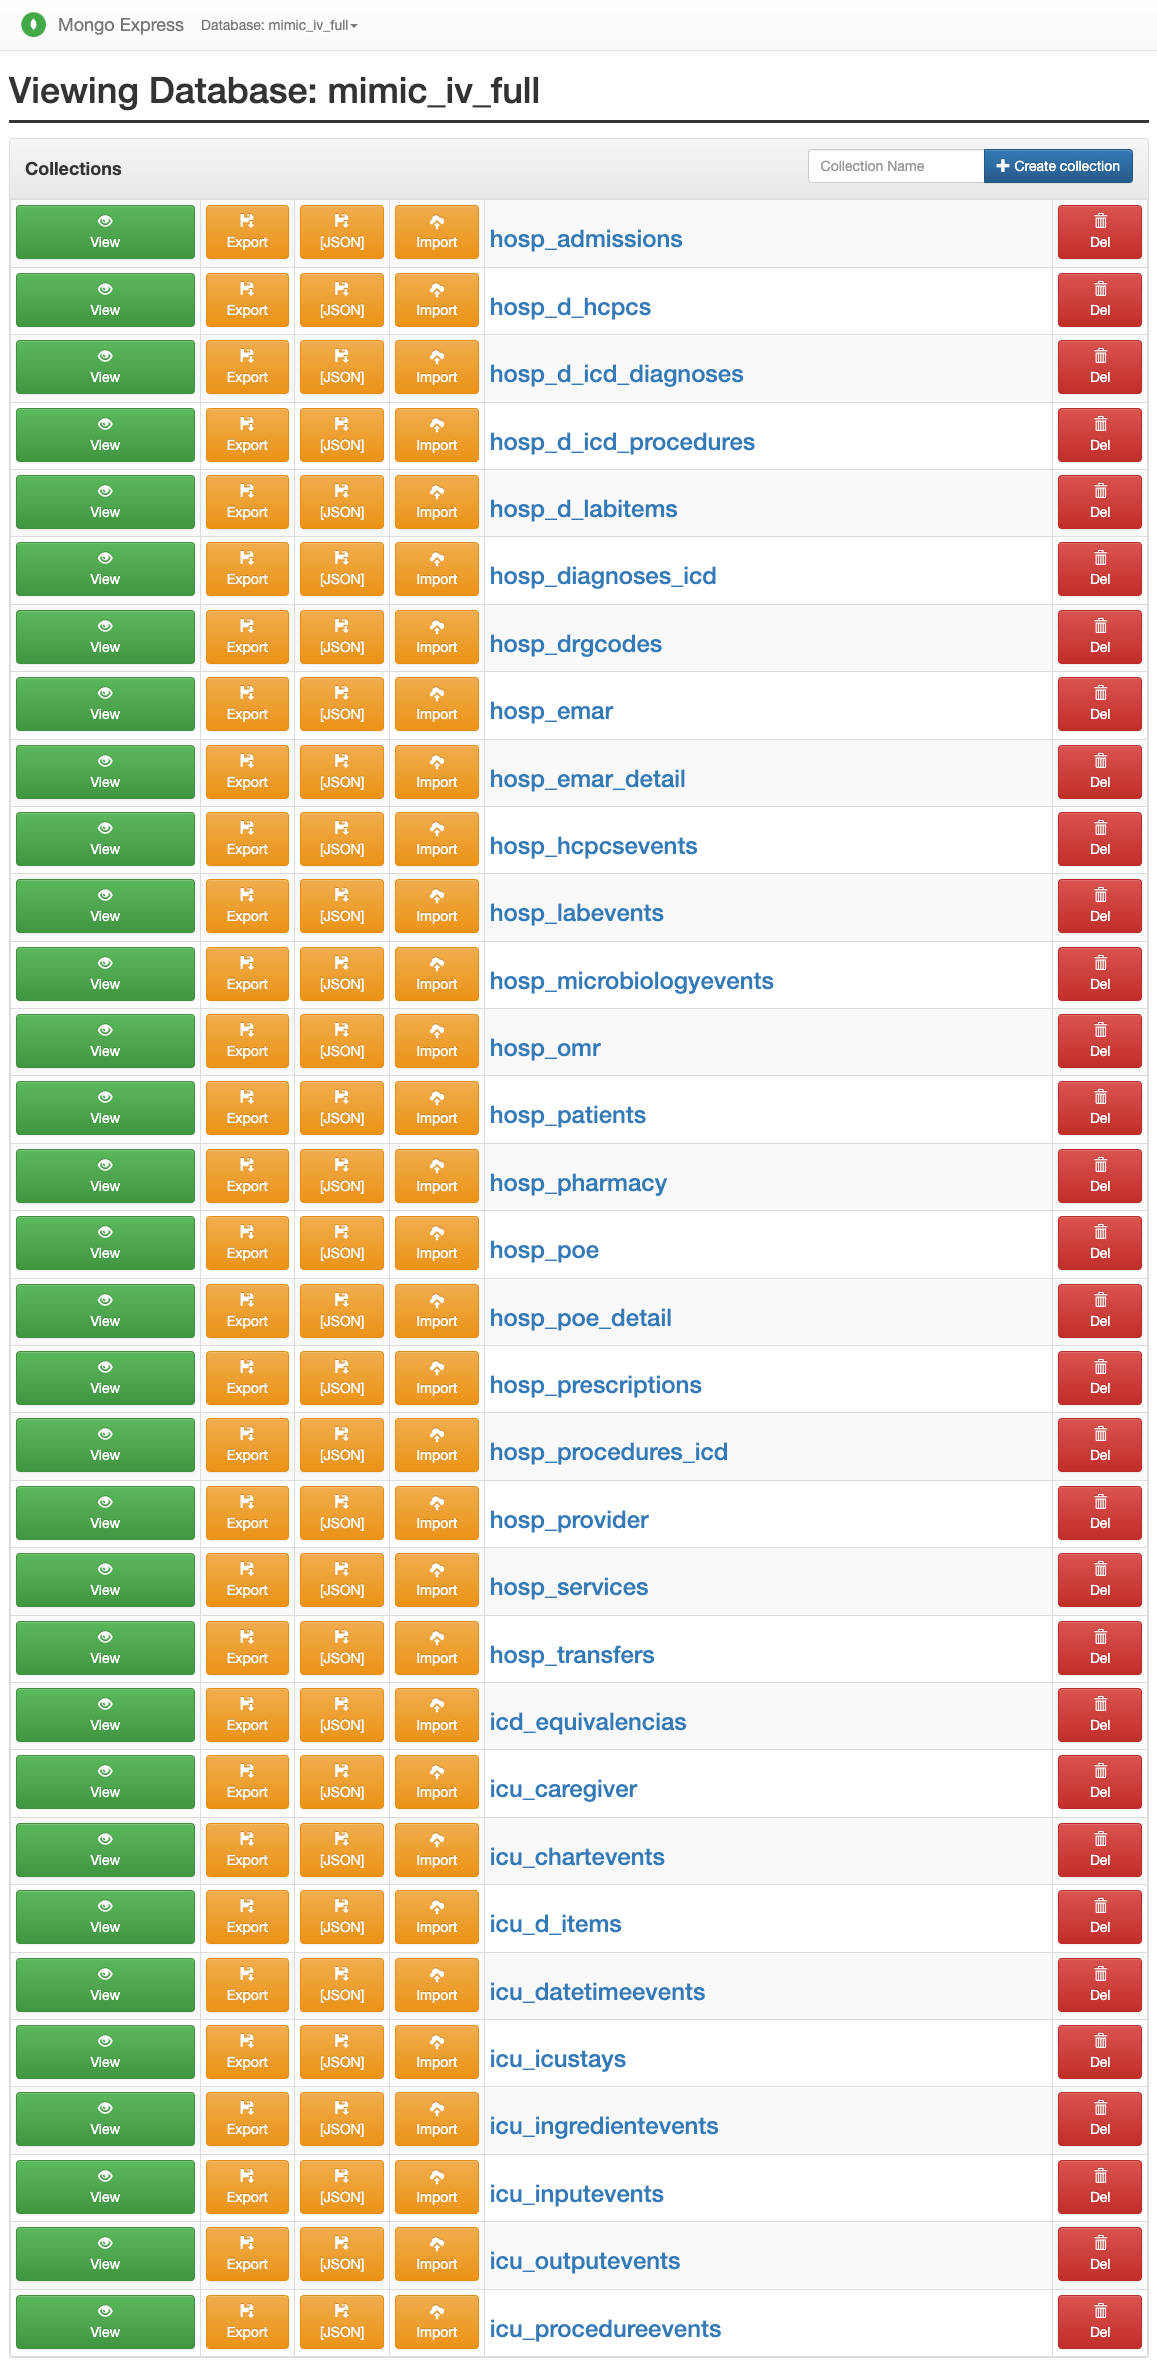
\includegraphics[width=0.8\textwidth]{imagenes/db_full_list.png}
    \caption{Colecciones resultantes tras la importacion. Captura de pantalla de la interfaz de Mongo Express.}
    \label{fig:db_full_list}
\end{figure}

\begin{figure}[H]
    \centering
    \fbox{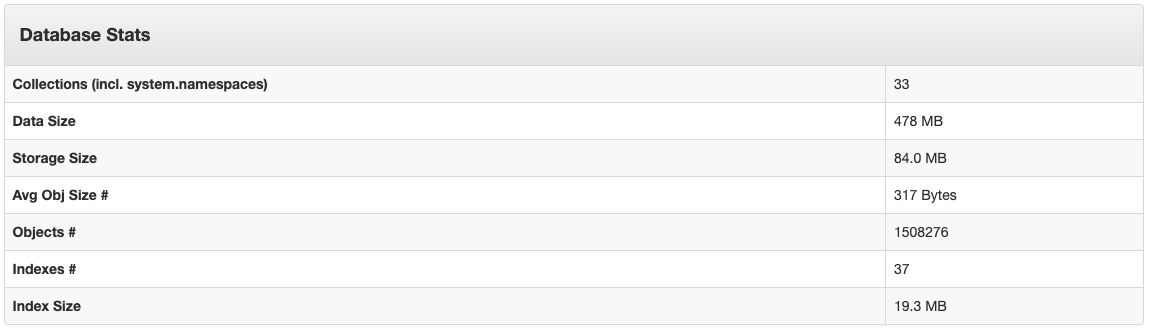
\includegraphics[width=1\textwidth]{imagenes/stats_demo.png}}
    %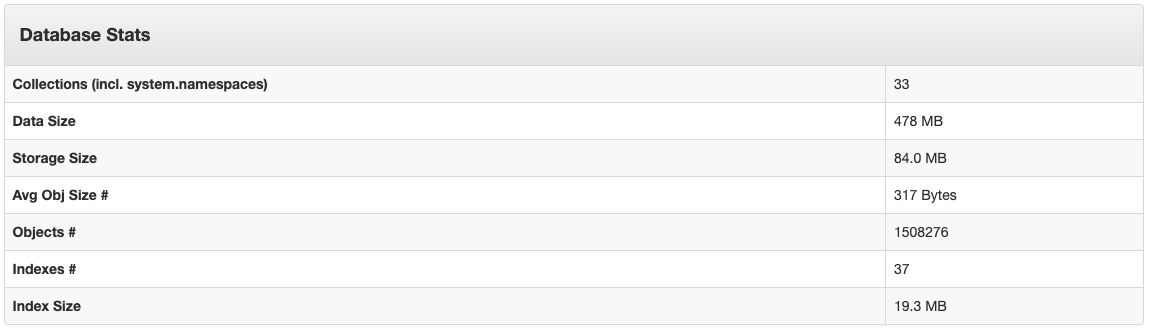
\includegraphics[width=1\textwidth]{imagenes/stats_demo.png}
    \caption{Estadísticas de la versión demo de la base de datos.}
    \label{fig:stats_demo}
\end{figure}

\begin{figure}[H]
    \centering
    \fbox{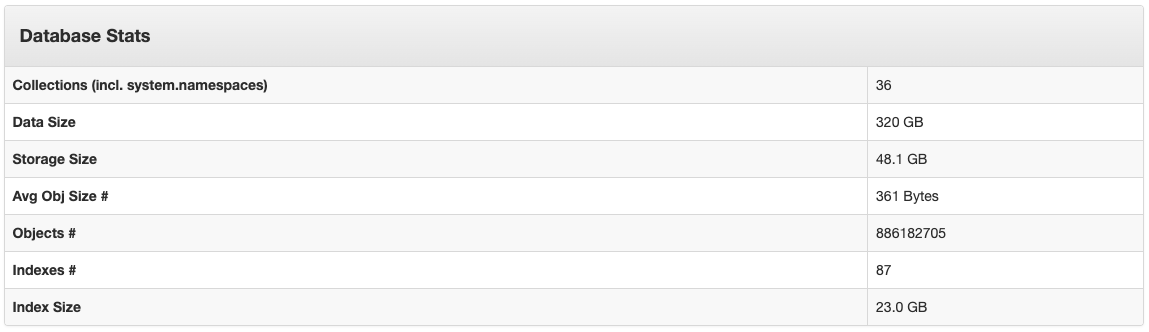
\includegraphics[width=1\textwidth]{imagenes/stats_full.png}}
    %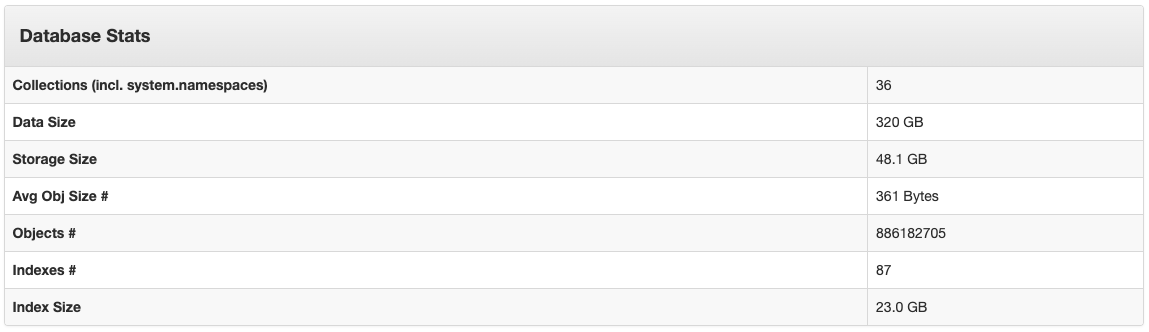
\includegraphics[width=1\textwidth]{imagenes/stats_full.png}
    \caption{Estadísticas de la versión completa de la base de datos.}
    \label{fig:stats_full}
\end{figure}


Además de las colecciones base que obtenemos de MIMIC-IV, a lo largo del proyecto se agregaron manualmente algunas más, necesarias tanto para pruebas como para algunas visualizaciones, de las que se hablará más tarde. Por eso, las estadísticas mostradas en las dos figuras anteriores, no coinciden exactamente con las del estado inicial del proyecto. 

También se crearon manualmente múltiples índices para optimizar el rendimiento de las consultas. Los índices en MongoDB funcionan de manera similar a los índices de un libro: crean estructuras de datos ordenadas que permiten localizar documentos específicos sin tener que examinar toda la colección. Esto es especialmente crítico en MIMIC-IV debido al volumen masivo de datos, donde algunas colecciones como \texttt{icu\_chartevents} contienen decenas de millones de registros. Por ejemplo, se crearon índices sobre campos clave como \texttt{subject\_id} (para consultas por paciente), \texttt{hadm\_id} (para ingresos hospitalarios), \texttt{charttime} (para búsquedas temporales) y \texttt{itemid} (para tipos específicos de mediciones). Sin estos índices, una consulta que busque todos los signos vitales de un paciente específico tendría que examinar millones de documentos, mientras que con el índice correspondiente la búsqueda se realiza en milisegundos.


En resumen, con esta implementación, se ha logrado transformar exitosamente el conjunto de datos MIMIC-IV desde su formato original en archivos CSV a una base de datos MongoDB completamente funcional y optimizada. La combinación de una estructura de datos bien comprendida, índices estratégicamente ubicados y colecciones auxiliares especializadas proporciona una base sólida para el procesamiento eficiente de consultas complejas sobre grandes volúmenes de datos clínicos. Esta infraestructura de datos establece los cimientos para el siguiente componente del sistema: la API RESTful que permitirá acceder, procesar y servir esta información de manera estructurada y escalable.





%Por ejemplo, el número total de colecciones esperado al comienzo es de 32 (22 del módulo \texttt{hosp}, 9 del módulo \texttt{icu} y 1 de \texttt{icd\_equivalencias}. 
%@todo: en que punto voy a hablar de las colecciones nuevas que he añadido yo -> aqui mismo -> NO, cuando hable de cada visualizacion



%\begin{figure}[H]
%  \centering
%  \fbox{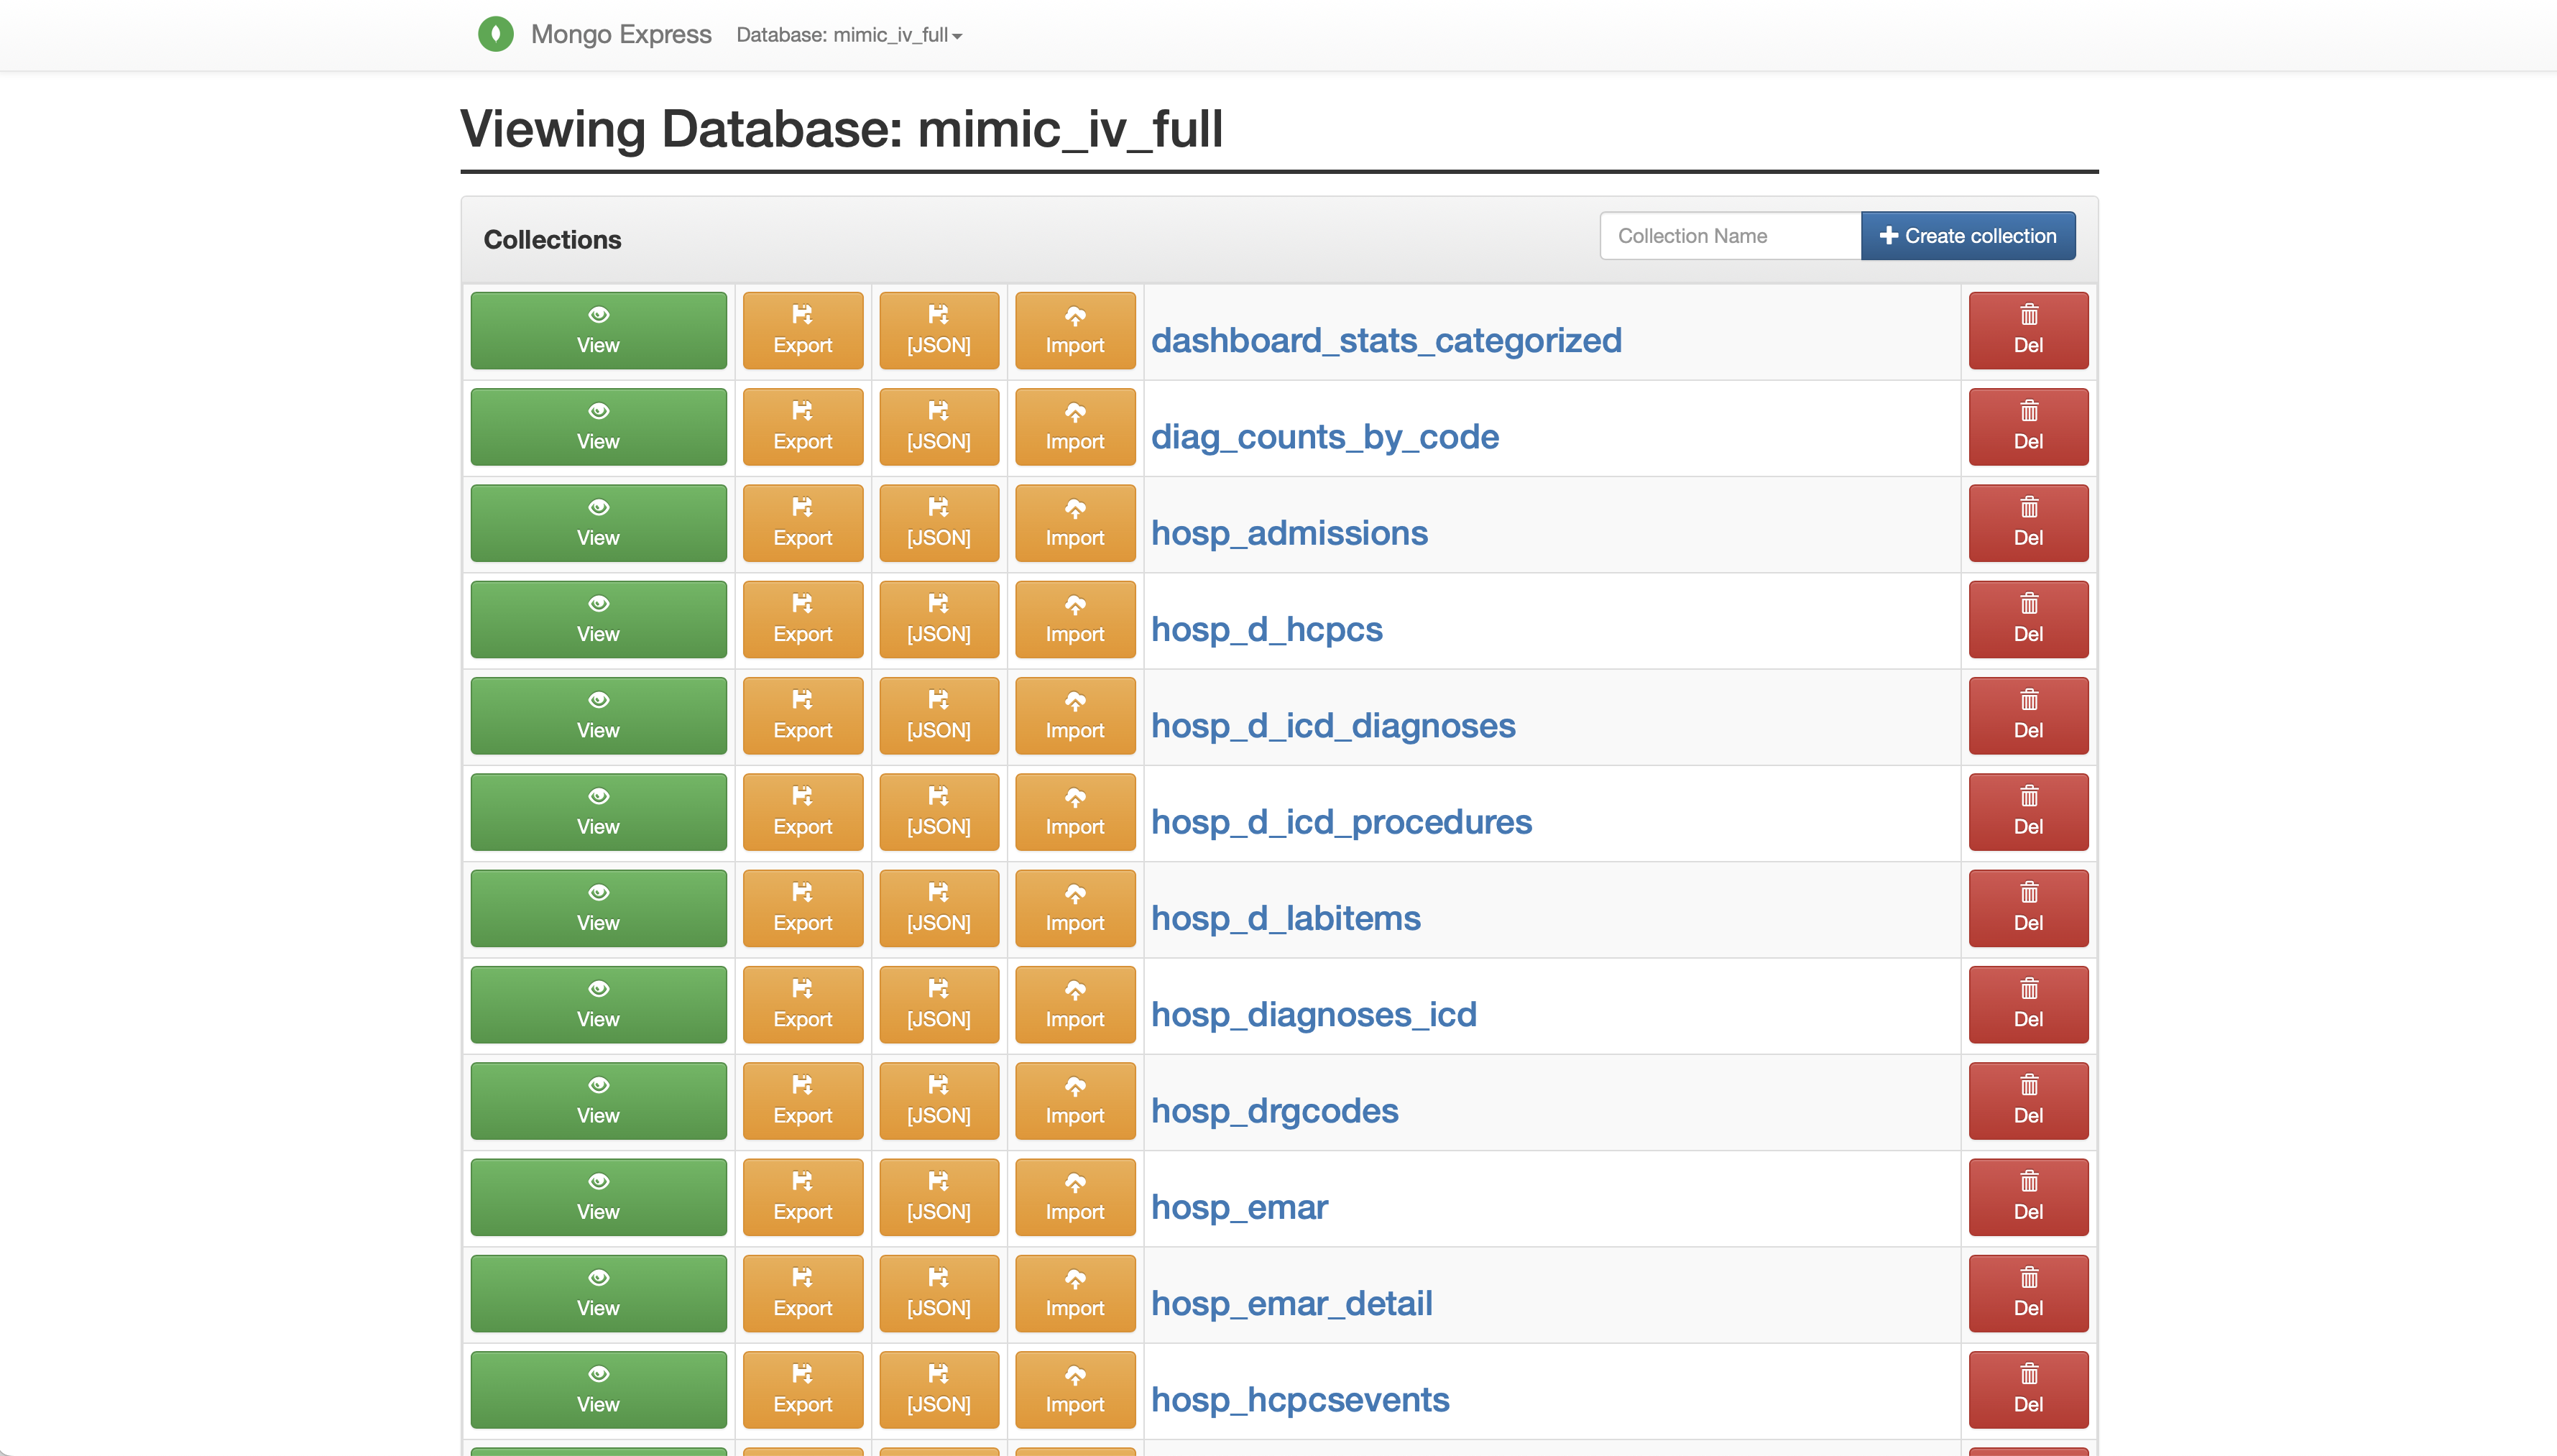
\includegraphics[width=1\textwidth]{imagenes/screenshot2.png}}
%  \caption{Captura de pantalla de Mongo Express}
%  \label{fig:screenshot2}
%\end{figure}


\subsection{API RESTful}

La API que obtiene, procesa y sirve los datos está construida sobre FastAPI \cite{fastapi}, un framework moderno que combina alto rendimiento con una sintaxis intuitiva y generación automática de documentación. Para separar responsabilidades, el código se estructura de la siguiente forma:

\begin{itemize}
\item \textbf{Capa de utilidades:} El módulo \texttt{utils/mongo.py} encapsula la conexión a MongoDB y proporciona funciones de utilidad, y \texttt{utils/mcp.py} contiene el código para el servidor MCP.
\item \textbf{Capa de rutas:} Organizadas por funcionalidad en el directorio \texttt{routes/}, incluyen endpoints para pacientes, dashboard, gráficos y chat.
\item \textbf{Capa de aplicación:} El archivo principal \texttt{main.py} configura la aplicación, middleware CORS y el enrutamiento.
\end{itemize}

Utilizamos Uvicorn \cite{uvicorn} como servidor que escuchará las peticiones a los endpoints. La API está estructurada modularmente mediante routers de FastAPI, organizados por funcionalidad:

\textbf{Endpoints de pacientes (\texttt{/api/patients}):}
\begin{itemize}
\item \texttt{GET /api/patients/\{subject\_id\}}: Obtiene información completa de un paciente específico mediante múltiples agregaciones MongoDB que incluyen datos demográficos, historial de ingresos, diagnósticos con descripciones ICD, procedimientos y eventos de laboratorio agrupados por ingreso.
\item \texttt{HEAD /api/patients/\{subject\_id\}/exists}: Verificación rápida de existencia de paciente (HTTP 200/404).
%\item \texttt{GET /api/patients/}: Lista los primeros pacientes disponibles del dataset demo.
\end{itemize}


\newpage
\textbf{Endpoints del dashboard (\texttt{/api/dashboard}):}
\begin{itemize}
\item \texttt{GET /api/dashboard/stats}: Obtiene estadísticas categorizadas pre-calculadas desde la colección \texttt{dashboard\_stats\_categorized} para máximo rendimiento, organizadas en cinco categorías: Demographics \& Admissions, Diagnoses \& Procedures, ICU Care, Lab \& Medications, y Hospital Flows.
\end{itemize}

\textbf{Endpoints de gráficos (\texttt{/api/charts}):}
\begin{itemize}
\item \texttt{GET /api/charts/admission-heatmap}: Genera datos para mapas de calor de ingresos hospitalarios con opciones de filtrado y vistas horarias/mensuales.
\item \texttt{GET /api/charts/age-distribution}: Distribución de pacientes por edad y género para pirámides poblacionales.
\item \texttt{GET /api/charts/icu-stay-duration}: Duración promedio de estancias en UCI por unidad.
\item \texttt{GET /api/charts/diagnosis-icicle}: Datos para diagramas icicle de diagnósticos categorizados.
\item \texttt{GET /api/charts/medications-sunburst}: Visualización sunburst de medicamentos prescritos por vía.
\item \texttt{GET /api/charts/hospital-transfers-chord}: Datos para diagramas chord de transferencias hospitalarias.
\end{itemize}

\textbf{Endpoints de inteligencia artificial:}
\begin{itemize}
\item \texttt{POST /chat/}: Interfaz de chat con streaming response que integra OpenAI GPT-5 con herramientas MCP para consultas en lenguaje natural sobre datos MIMIC-IV.
\item \texttt{POST /api/summary/patient}: Genera resúmenes clínicos automatizados utilizando OpenAI GPT-4.1.
\end{itemize}

\textbf{Endpoints de monitoreo:}
\begin{itemize}
\item \texttt{GET /health}: Verificación de estado del servidor.
\item \texttt{GET /}: Endpoint raíz con información básica de la API.
\end{itemize}

\newpage
\subsection{Inteligencia Artificial}

La integración de inteligencia artificial en esta plataforma se fundamenta en la utilización de grandes modelos de lenguaje (LLMs) para facilitar la consulta y análisis de datos clínicos en lenguaje natural. Esta aproximación permite que usuarios sin conocimientos técnicos avanzados puedan extraer información valiosa de la base de datos MIMIC-IV mediante conversaciones naturales, eliminando la barrera técnica que tradicionalmente requería conocimientos de SQL o programación.

Para este proyecto se ha elegido trabajar con los modelos de texto de OpenAI, específicamente GPT-4.1, accedido mediante su API oficial para Python. Este modelo presentado por OpenAI en abril de 2025, representa una evolución significativa respecto a sus predecesores. Cuenta con una ventana de contexto ampliada de hasta 1 millón de tokens, superando significativamente los 128.000 tokens de modelos previos como GPT-4o, pero también modelos nuevos como GPT-5, que tiene una ventana de 400.000 tokens. Esta capacidad expandida permite procesar y analizar grandes volúmenes de información médica en una sola interacción, facilitando el análisis de múltiples registros clínicos, documentos extensos y conversaciones prolongadas sin perder coherencia ni relevancia contextual, y es principalmente ese el motivo de su elección.

\subsubsection{Model Context Protocol (MCP)}

Una de las innovaciones técnicas más relevantes incorporadas en este proyecto es la implementación del Model Context Protocol (MCP), un estándar abierto desarrollado por Anthropic y presentado en noviembre de 2024 \cite{AnthropicMCP2024}. MCP surge como respuesta a uno de los principales desafíos en el desarrollo de sistemas de inteligencia artificial: la integración estandarizada y segura entre modelos de lenguaje de gran tamaño y fuentes de datos externas.


Tradicionalmente, la conexión entre modelos de IA y bases de datos requería el desarrollo de integraciones personalizadas para cada caso específico. Técnicas como RAG (Retrieval-Augmented Generation), aunque efectivas para enriquecer las respuestas de los modelos con información externa, demandaban implementaciones ad-hoc para cada fuente de datos. Esta aproximación resultaba en arquitecturas complejas, propensas a errores y difíciles de mantener. Cada nueva fuente de datos o herramienta externa requería desarrollo personalizado, generando fragmentación tecnológica y duplicación de esfuerzos. MCP aborda estos problemas proporcionando una interfaz universal que estandariza la comunicación entre sistemas de IA y recursos externos, incluyendo bases de datos, APIs, sistemas de archivos y herramientas especializadas.

\begin{figure}[H]
  \centering
  \fbox{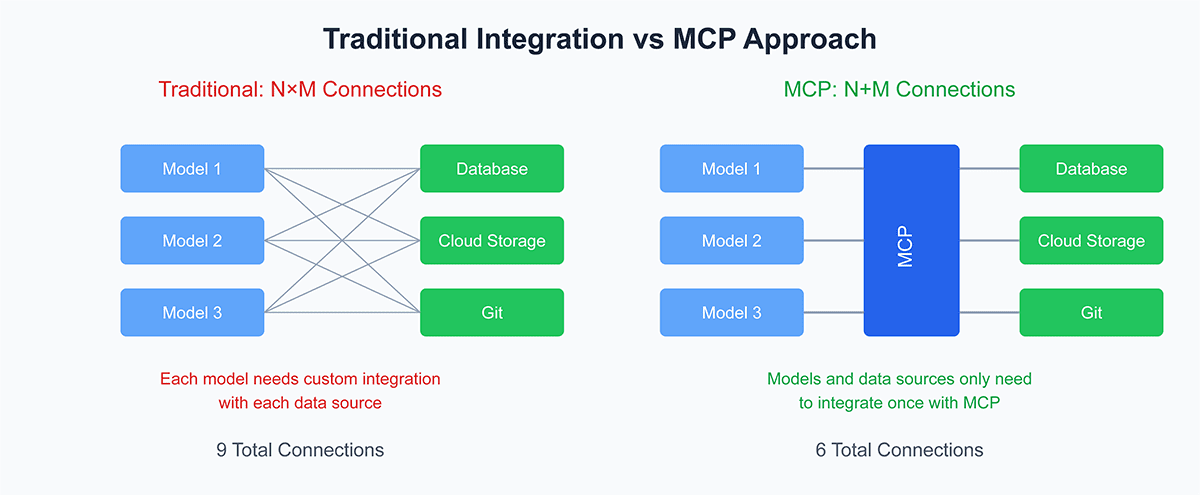
\includegraphics[width=1\textwidth]{imagenes/mcp1.jpg}}
  %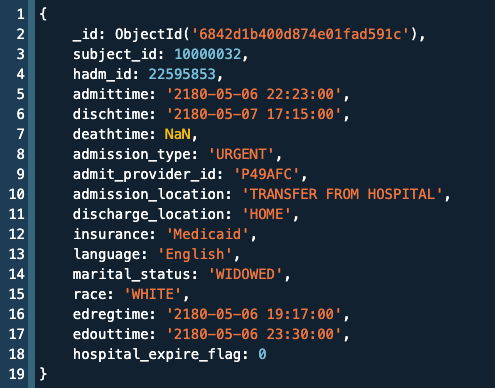
\includegraphics[width=0.6\textwidth]{imagenes/ej_admission.png}
  \caption{Integración tradicional vs el enfoque MCP \cite{mcp1foto}.}
  \label{fig:mcp1}
\end{figure}


MCP opera bajo una arquitectura cliente-servidor compuesta por tres componentes principales \cite{mcp_arch}:

\begin{itemize}
\item \textbf{MCP Host:} La aplicación principal que requiere acceso a datos externos, como una interfaz de chat impulsada por IA o un entorno de desarrollo integrado.
\item \textbf{MCP Client:} Un componente que mantiene una conexión dedicada con un servidor MCP específico y obtiene contexto de dicho servidor para que lo utilice el host MCP. Cada cliente mantiene una relación uno-a-uno con su servidor correspondiente.
\item \textbf{MCP Server:} Programas especializados que se conectan a fuentes de datos específicas y exponen funcionalidades a través del protocolo MCP estandarizado.
\end{itemize}

\begin{figure}[H]
  \centering
  \fbox{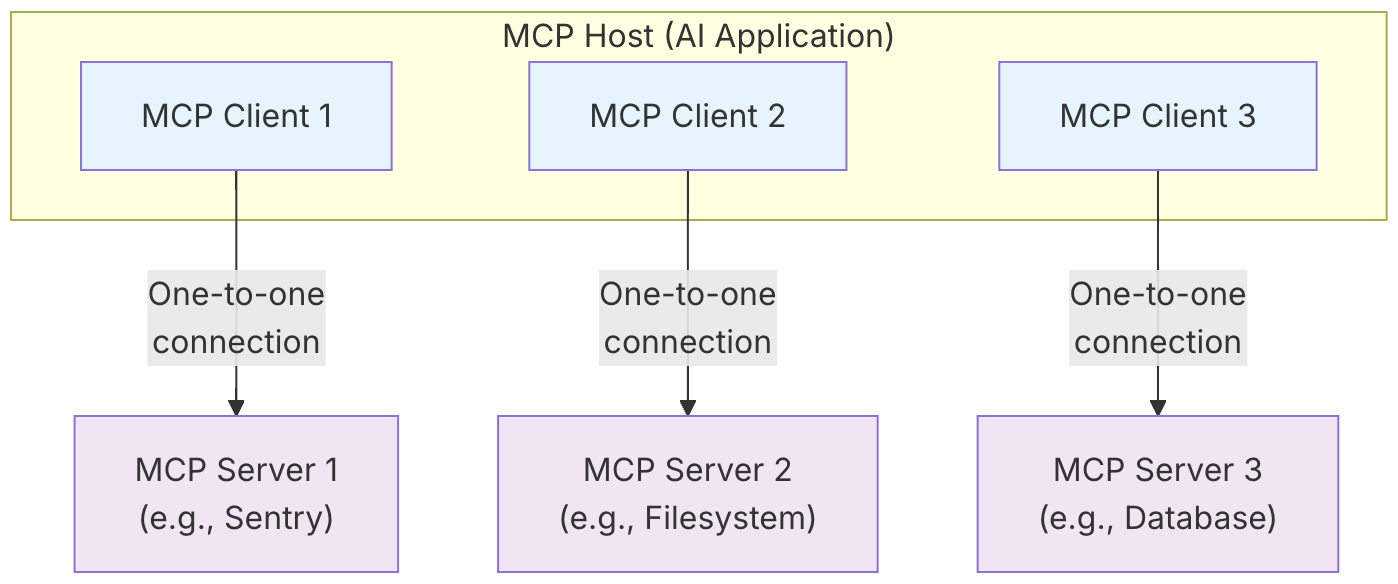
\includegraphics[width=1\textwidth]{imagenes/mcp2.png}}
  %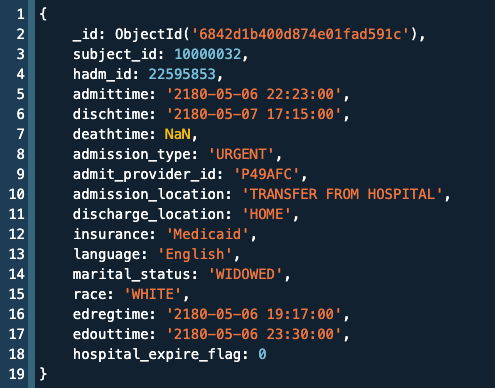
\includegraphics[width=0.6\textwidth]{imagenes/ej_admission.png}
  \caption{Arquitectura MCP.}
  \label{fig:mcp2}
\end{figure}

El flujo de comunicación se inicia cuando el modelo de IA necesita acceder a información externa. El anfitrión envía una solicitud al cliente MCP, quien la encamina al servidor correspondiente. Este último procesa la petición, accede a los datos requeridos y devuelve la información siguiendo el protocolo establecido. Esta arquitectura modular garantiza que los modelos de IA tengan acceso a contexto actualizado y relevante sin comprometer la seguridad o integridad de los datos subyacentes.





En el contexto de esta plataforma, se ha desarrollado un servidor MCP especializado para interactuar con la base de datos MIMIC-IV almacenada en MongoDB. Para ello, se utilizó FastMCP \cite{fastmcp}, un framework Python diseñado específicamente para simplificar la creación de servidores que implementan el Model Context Protocol. Con esta herramienta, nuestra tarea únicamente se reduce a definir las herramientas a las que podrán acceder los LLMs. En nuestro caso, se han implementado las siguientes seis herramientas que permiten la interacción con la base de datos:

\begin{itemize}
\item \texttt{get\_schema}: Obtiene la estructura de cualquier colección MongoDB, permitiendo al modelo entender los campos disponibles y sus tipos de datos.
\item \texttt{find\_documents}: Realiza consultas directas sobre documentos específicos, aplicando filtros y limitaciones de resultados.
\item \texttt{aggregate\_data}: Ejecuta pipelines de agregación MongoDB para análisis complejos y cálculos estadísticos.
\item \texttt{count\_documents}: Proporciona conteos rápidos de documentos que cumplen criterios específicos.
\item \texttt{list\_collections}: Enumera todas las colecciones disponibles en la base de datos.
\item \texttt{get\_indexes}: Obtiene información sobre índices de rendimiento de las colecciones.
\end{itemize}


\begin{figure}[H]
  \centering
  \fbox{
\includegraphics[width=0.4\textwidth]{imagenes/fastmpc.png}}
  %
\includegraphics[width=0.4\textwidth]{imagenes/fastmpc.png}
  \caption{Logo del framework FastMCP.}
  \label{fig:fastmcp}
\end{figure}



El servidor MCP se integra con el sistema principal montándose en el endpoint \texttt{/mcp} de la API principal.

%La adopción de MCP en esta plataforma aporta múltiples beneficios técnicos y funcionales:

%\textbf{Estandarización:} Elimina la necesidad de desarrollar interfaces propietarias para cada tipo de consulta, reduciendo significativamente la complejidad del código y el tiempo de desarrollo.

%\textbf{Escalabilidad:} La arquitectura modular facilita la incorporación de nuevas fuentes de datos o herramientas sin modificar el núcleo del sistema de IA.

%\textbf{Seguridad:} Cada servidor MCP gestiona sus propios permisos y controles de acceso, proporcionando una capa adicional de seguridad sin comprometer la funcionalidad.

%\textbf{Rendimiento:} Al proporcionar acceso directo y estructurado a los datos relevantes, el modelo puede generar respuestas más precisas y contextualizadas con menor latencia.

%\textbf{Interoperabilidad:} Al seguir un estándar abierto, el sistema puede integrarse con otras herramientas y plataformas que adopten MCP, facilitando la colaboración y extensibilidad.

%La implementación de MCP representa así un paso hacia la madurez tecnológica en el campo de la integración de sistemas de IA con infraestructuras de datos complejas, posicionando este proyecto como un ejemplo práctico de las mejores prácticas emergentes en el desarrollo de aplicaciones sanitarias inteligentes.

%(... hablar sobre tema legal de proteccion de datos... todaviia no se si se puede...)


\subsection{Despliegue}

Para la implementación del backend, era necesario considerar los importantes requisitos de hardware que impone el conjunto de datos MIMIC-IV. Específicamente, se requería almacenamiento considerable para albergar los múltiples gigabytes de información clínica, así como múltiples núcleos de procesamiento para gestionar eficientemente las consultas paralelas a la base de datos y las peticiones simultáneas de la API.

En lugar de alquilar un VPS (Virtual Private Server) con estas especificaciones técnicas, lo que representaría un coste económico significativo para un proyecto académico, se optó por utilizar un servidor personal disponible. Este servidor ejecuta Proxmox VE \cite{proxmox}, un hipervisor de código abierto basado en Debian que combina virtualización de máquinas (KVM) y contenedores (LXC), proporcionando una plataforma completa para la gestión de infraestructura virtualizada.


\begin{figure}[H]
  \centering
  \fbox{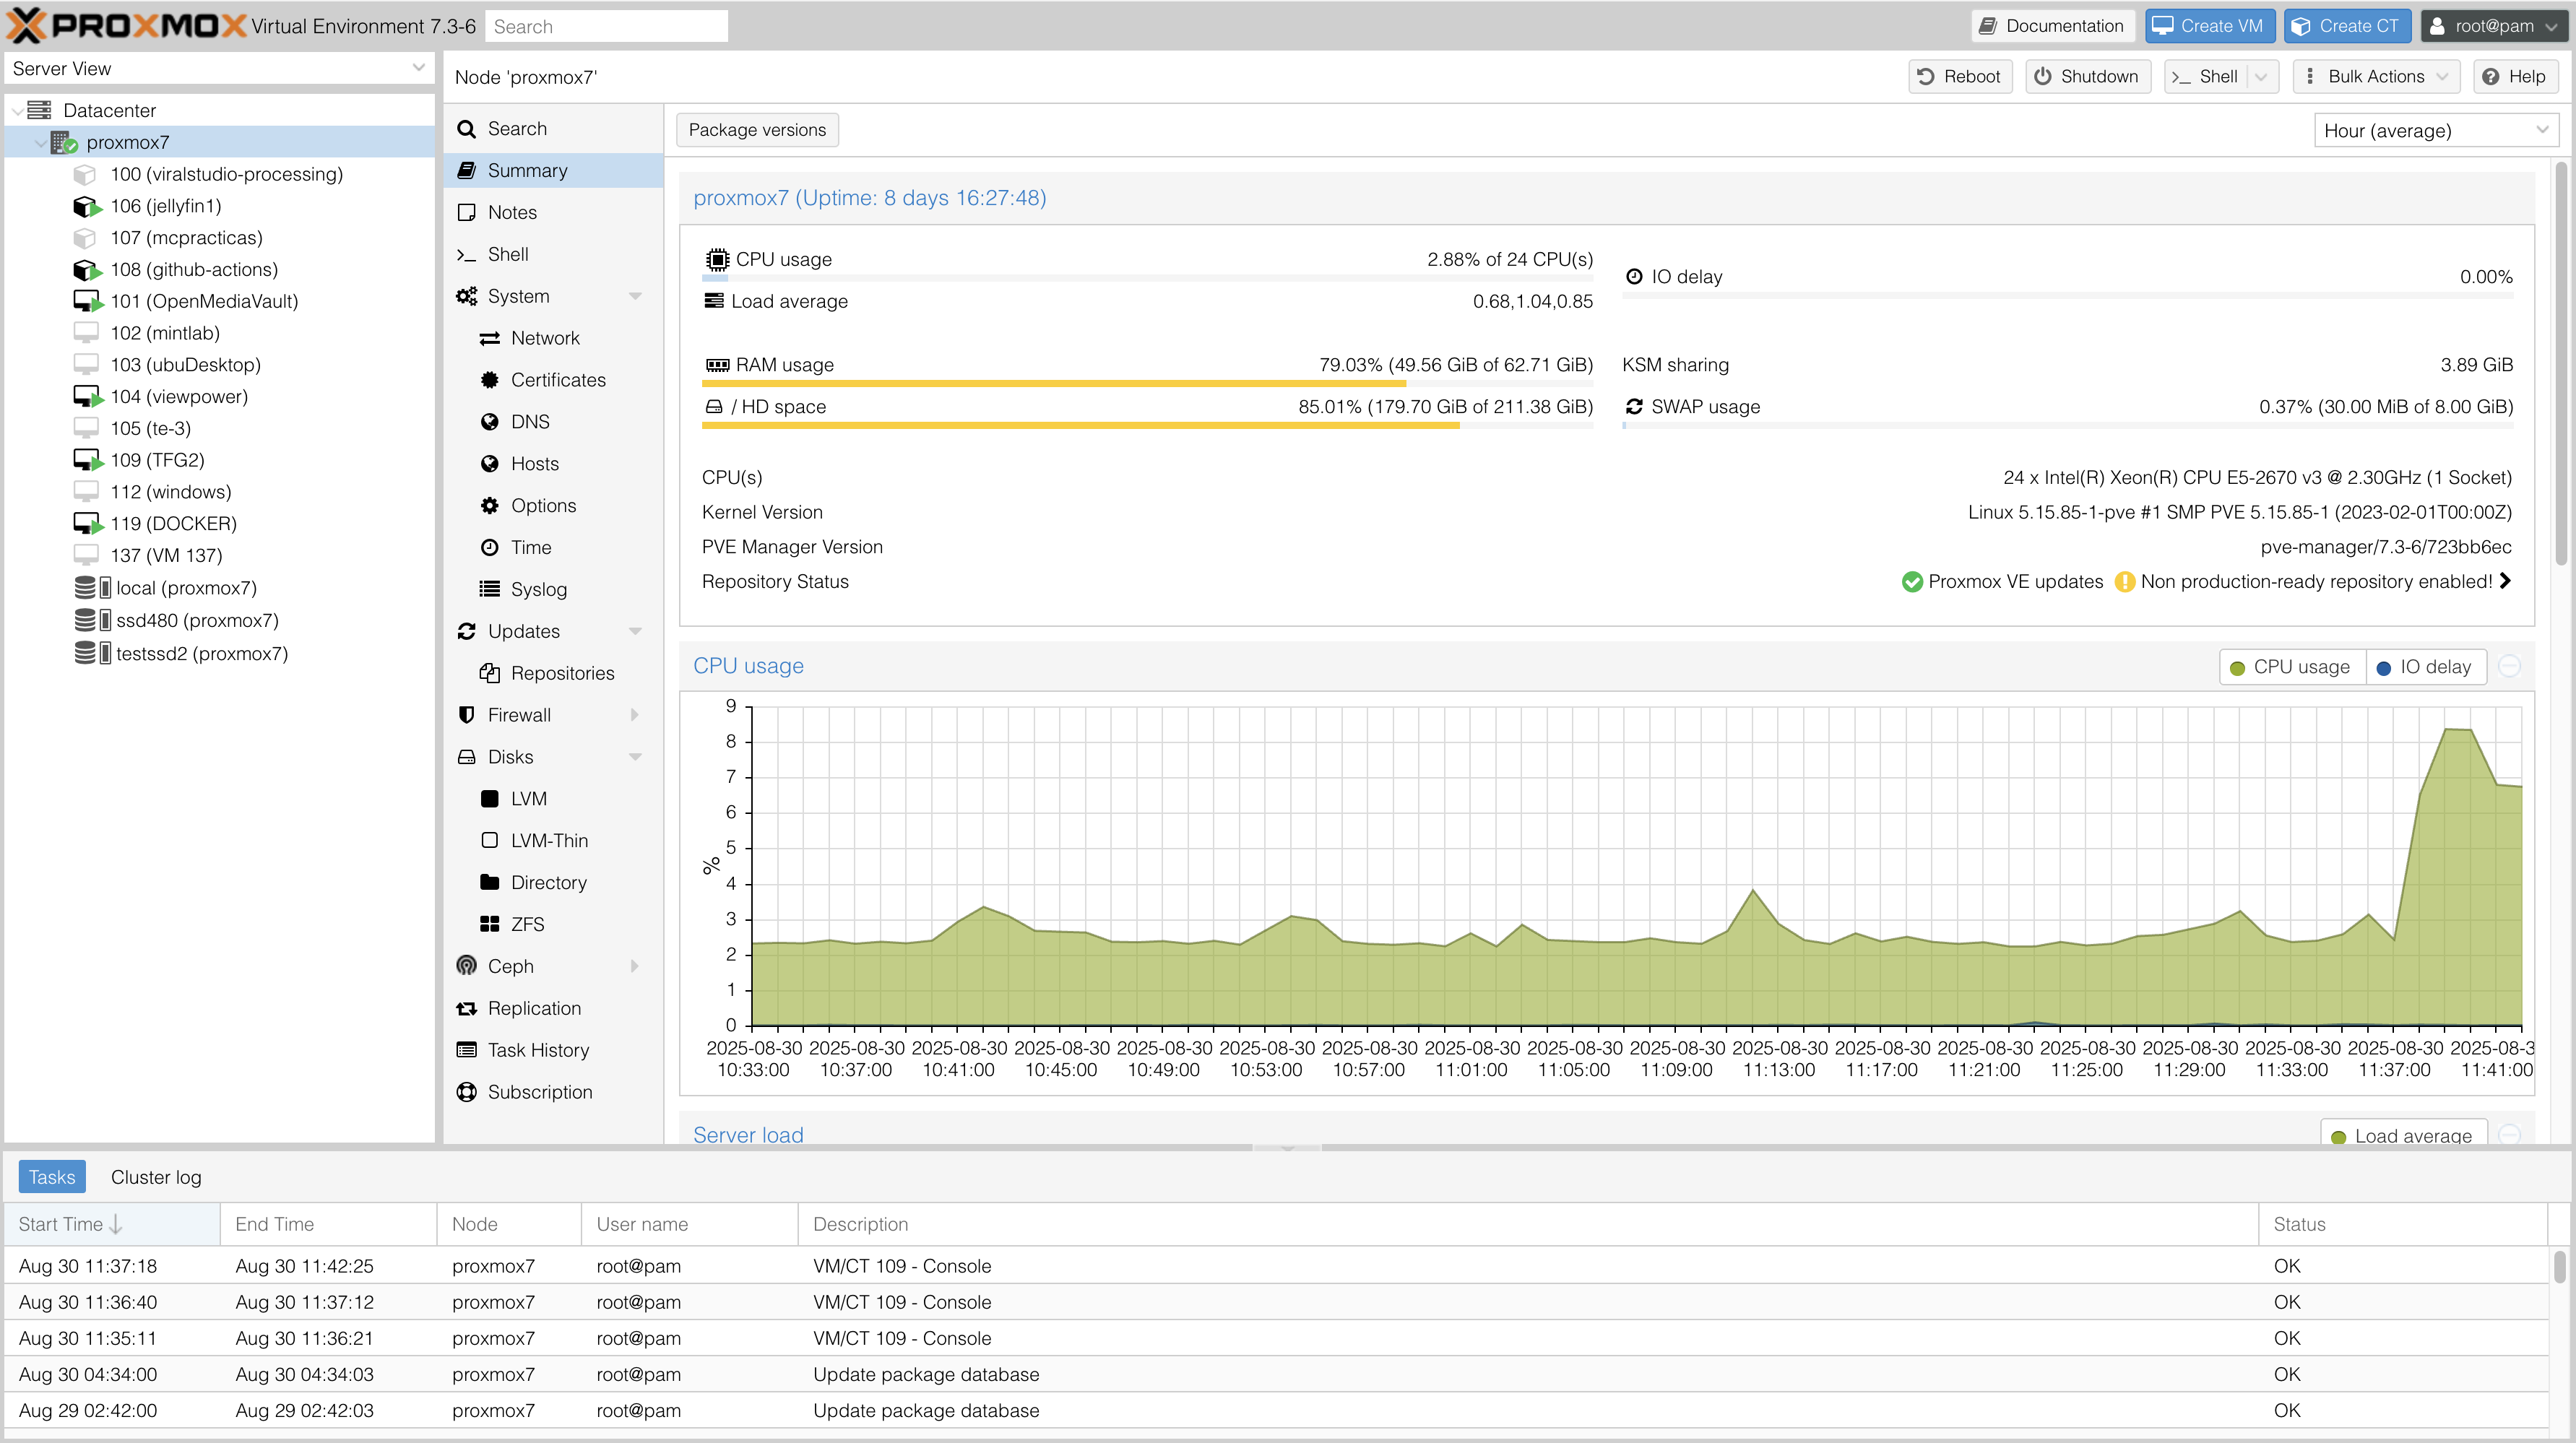
\includegraphics[width=1\textwidth]{imagenes/proxmox2.png}}
  %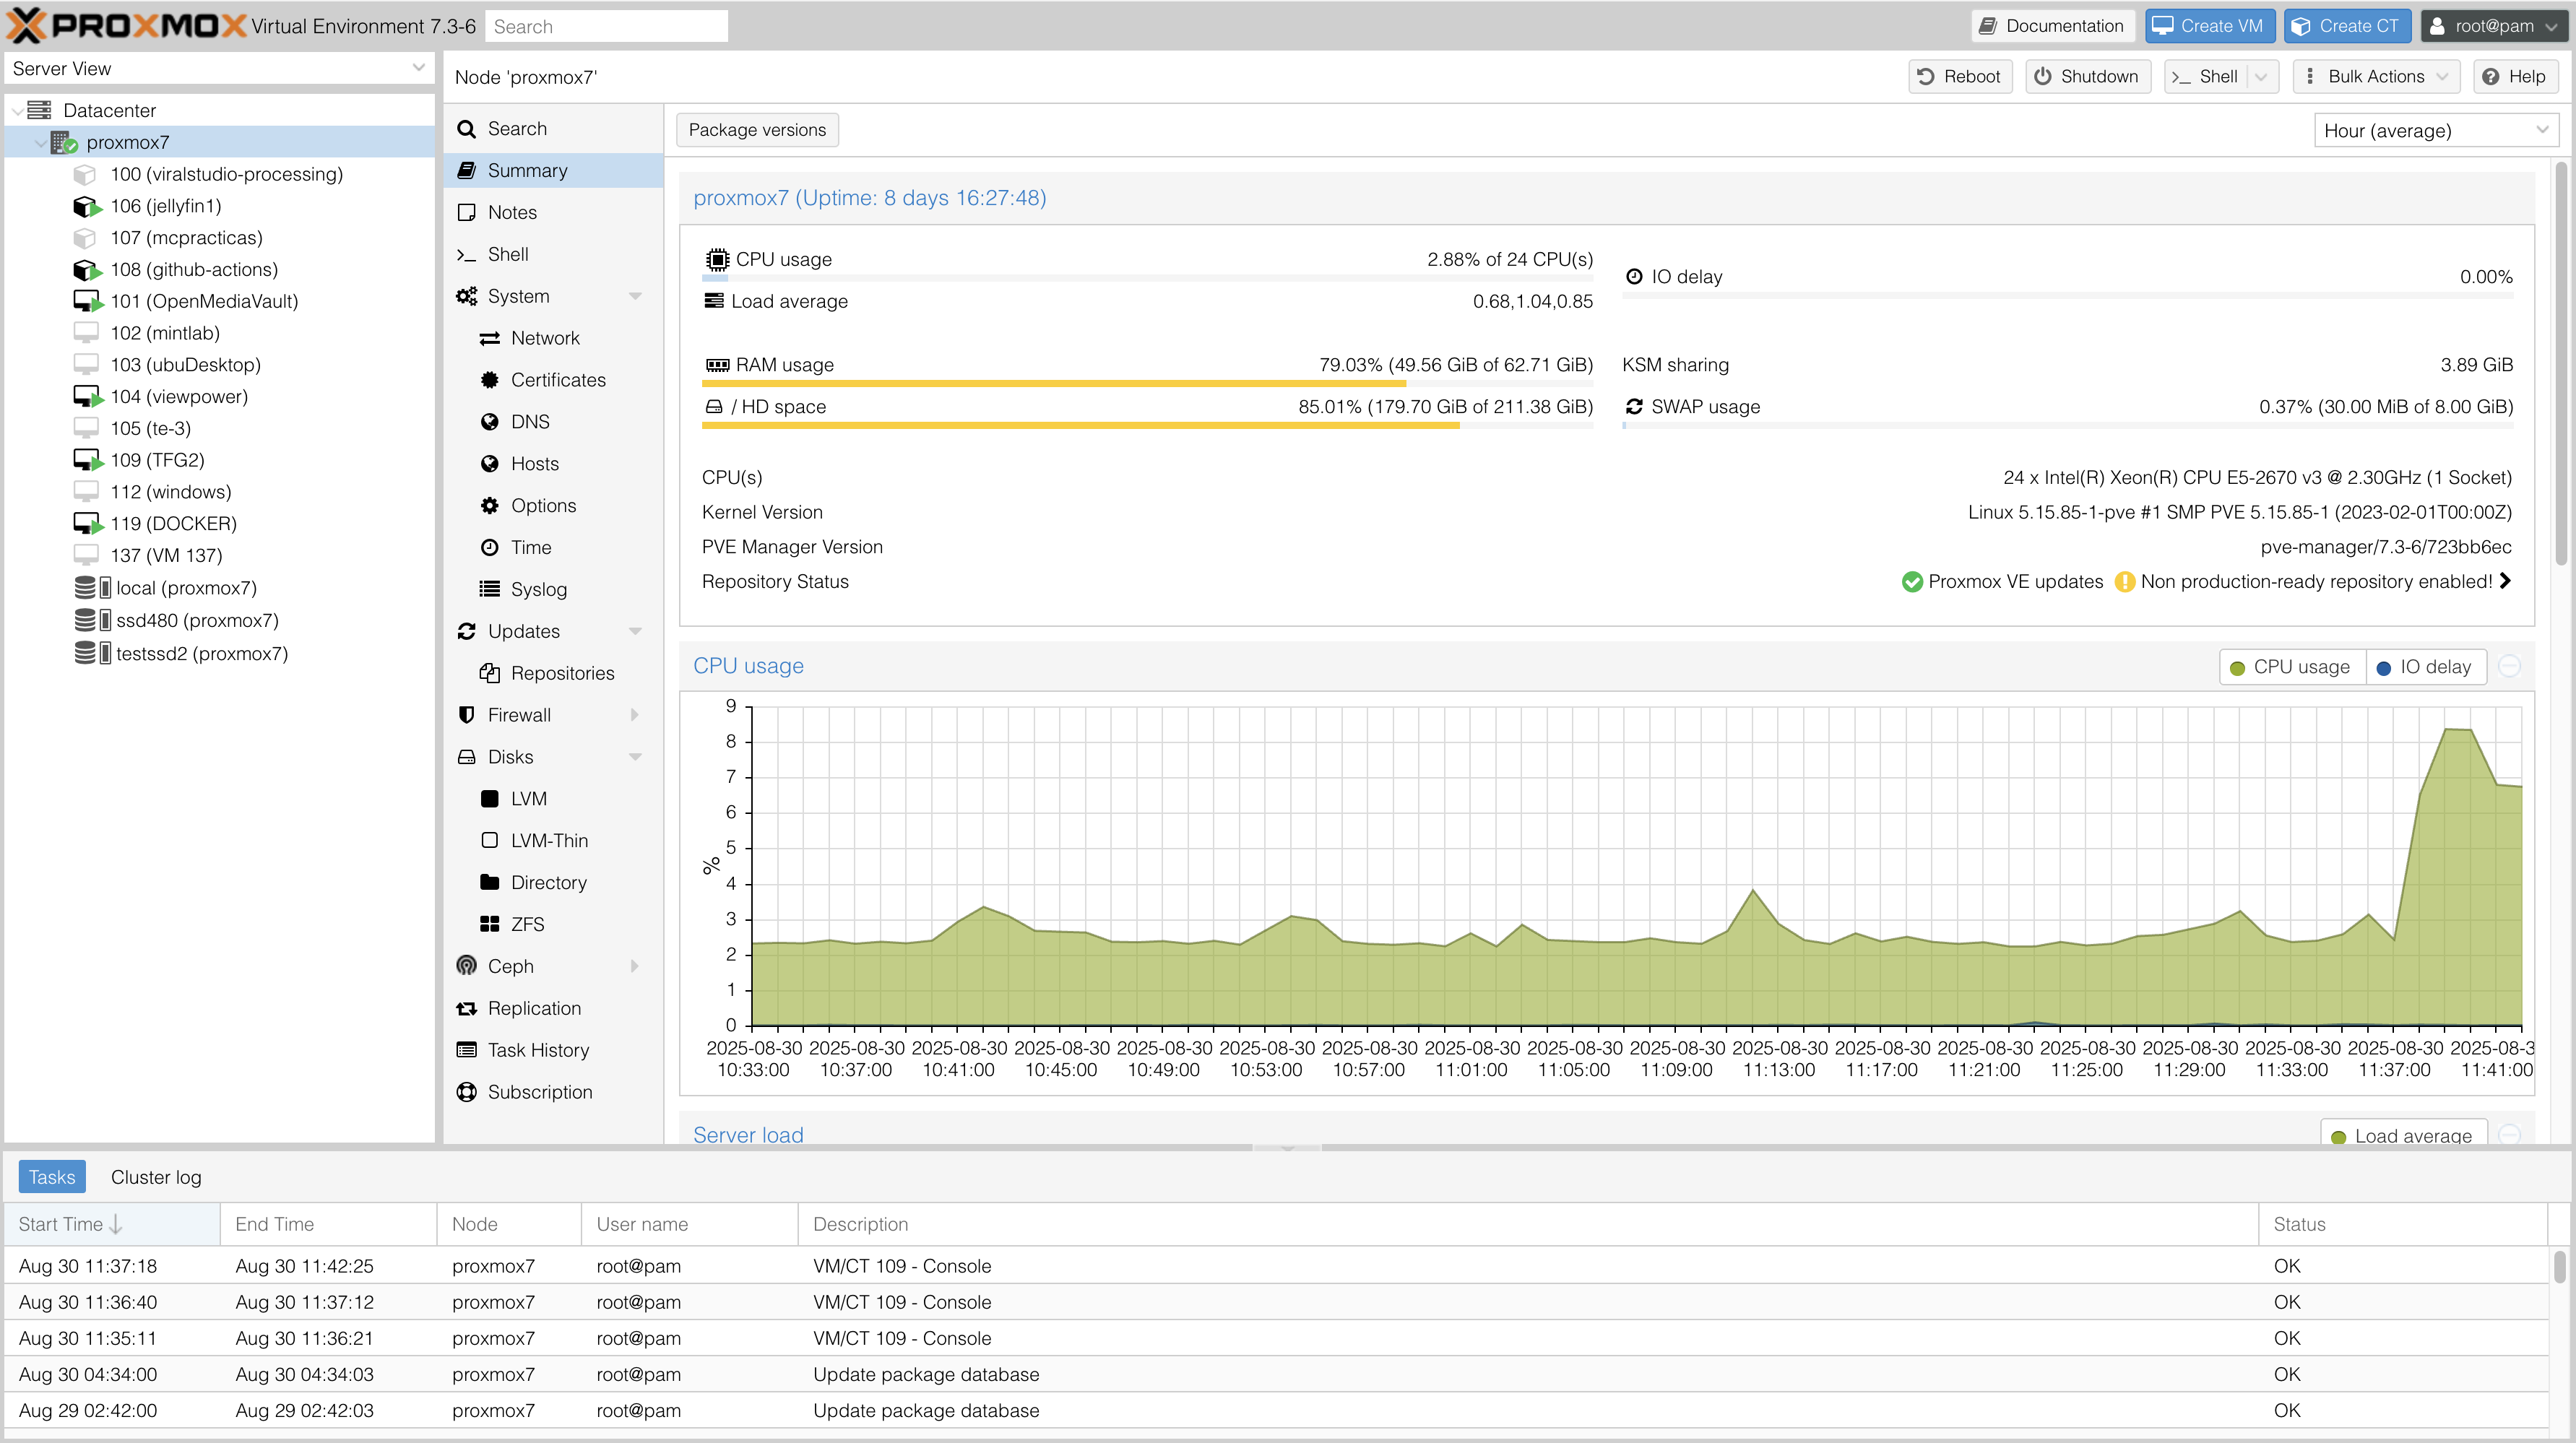
\includegraphics[width=1\textwidth]{imagenes/proxmox2.png}
  \caption{Captura de pantalla de la interfaz de Proxmox.}
  \label{fig:proxmox2}
\end{figure}



Se creó una máquina virtual con Ubuntu 24.04 Desktop como sistema operativo guest. Los recursos asignados a esta máquina virtual se fueron incrementando iterativamente según las necesidades observadas durante las pruebas de carga y la importación de datos. La configuración final establecida fue de 10 núcleos de CPU, 26 GB de memoria RAM y 128 GB de almacenamiento SSD, especificaciones que proporcionaron el rendimiento adecuado para gestionar tanto la base de datos MongoDB como la API.

Una vez que tanto la base de datos como la API funcionaban correctamente en el entorno local, era necesario desplegarlos para permitir el acceso público desde el frontend. Para esta tarea se utilizó Cloudflare Tunnels \cite{cloudflaretunnels}, que permite exponer servicios locales a Internet sin abrir puertos en el firewall ni configurar redirección de puertos. Cloudflare \cite{cloudflare} es una empresa que actúa como intermediario proporcionando servicios de CDN, DNS y seguridad web entre los usuarios finales y los servidores.

El despliegue se realizó mediante un contenedor Docker adicional que ejecuta el cliente \texttt{cloudflared}, estableciendo una conexión cifrada entre el servidor local y la infraestructura de Cloudflare. Esta implementación permite que la API sea accesible públicamente a través de un dominio o subdominio de nuestra elección, en nuestro caso \texttt{https://tfg-api.angeloyo.com}, proporcionando automáticamente certificados SSL/TLS, protección DDoS y optimizaciones de red.

Las principales ventajas de esta aproximación son su simplicidad y que mantiene el servidor completamente privado, ofreciendo una URL HTTPS estable consumible desde cualquier ubicación. Sin embargo, esta solución, aunque perfecta para el contexto de este TFG, no sería adecuada para entornos de producción profesionales donde se requerirían arquitecturas más robustas con balanceadores de carga, alta disponibilidad y redundancia geográfica.  


\begin{figure}[H]
  \centering
  \fbox{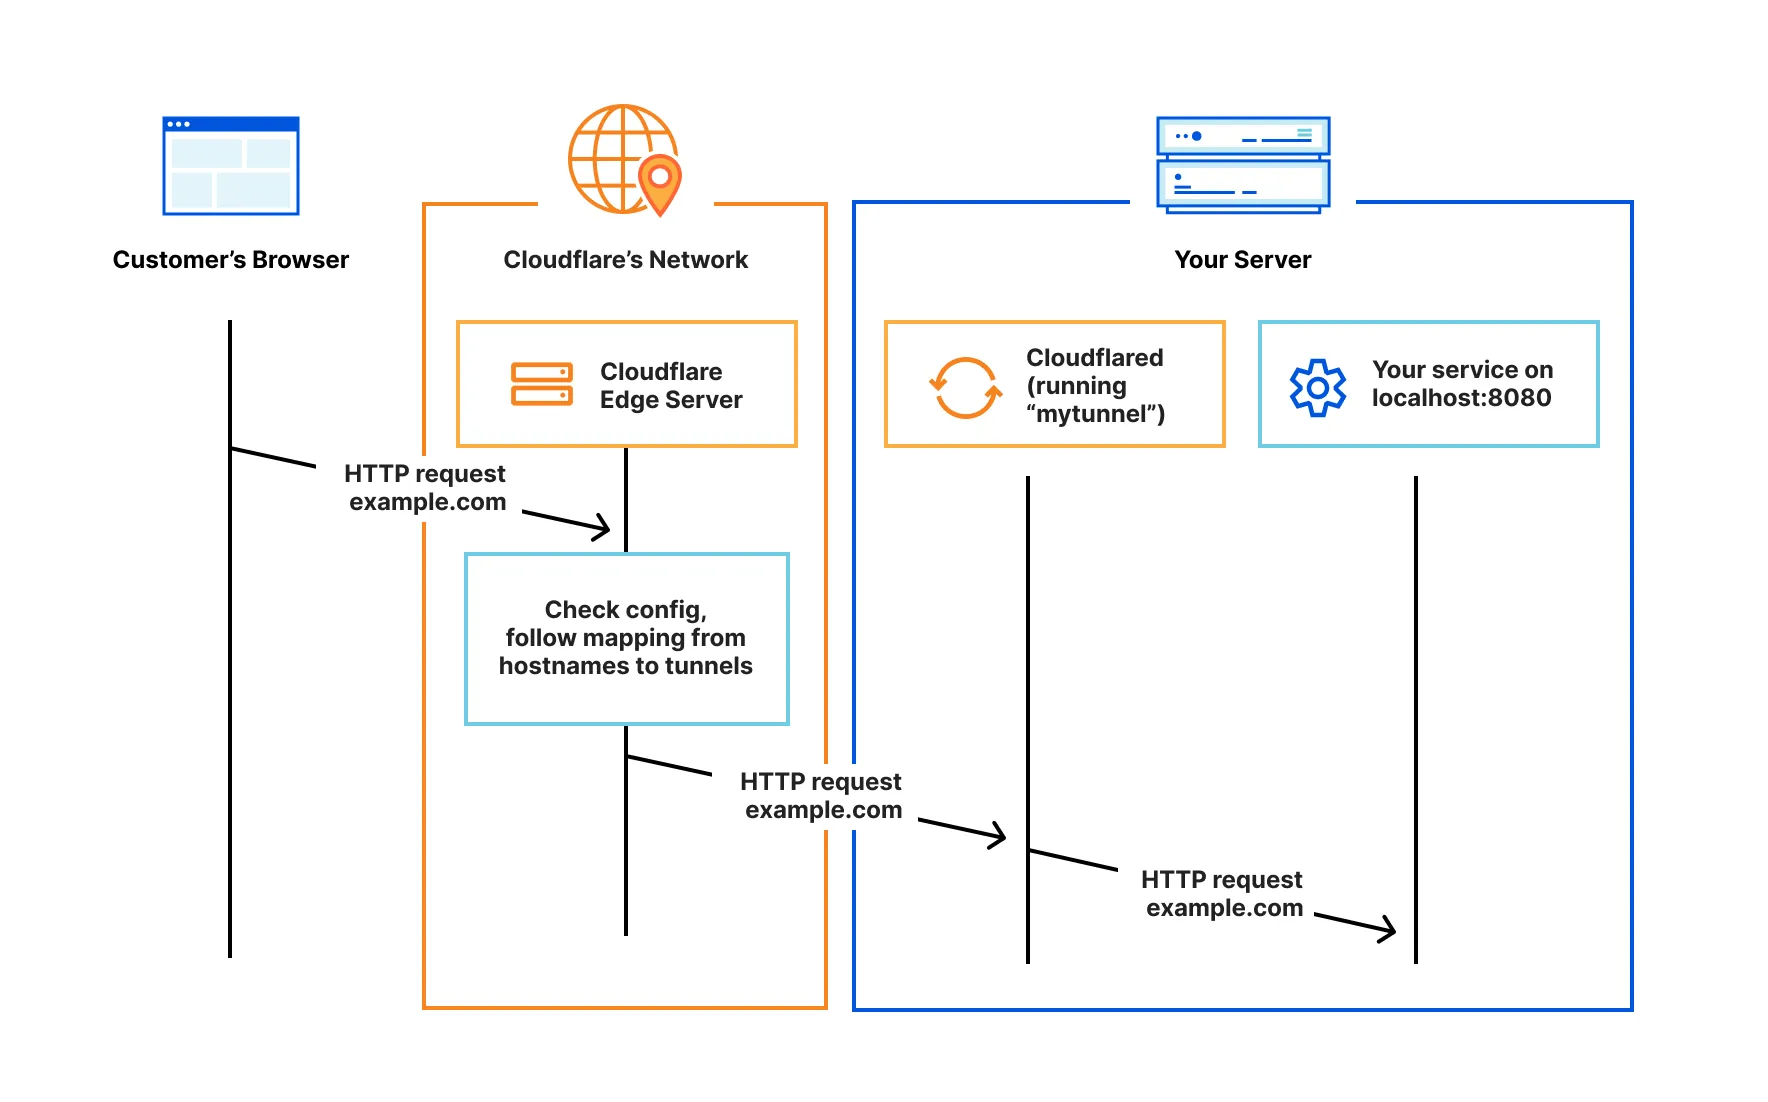
\includegraphics[width=1\textwidth]{imagenes/cloudflared.png}}
  %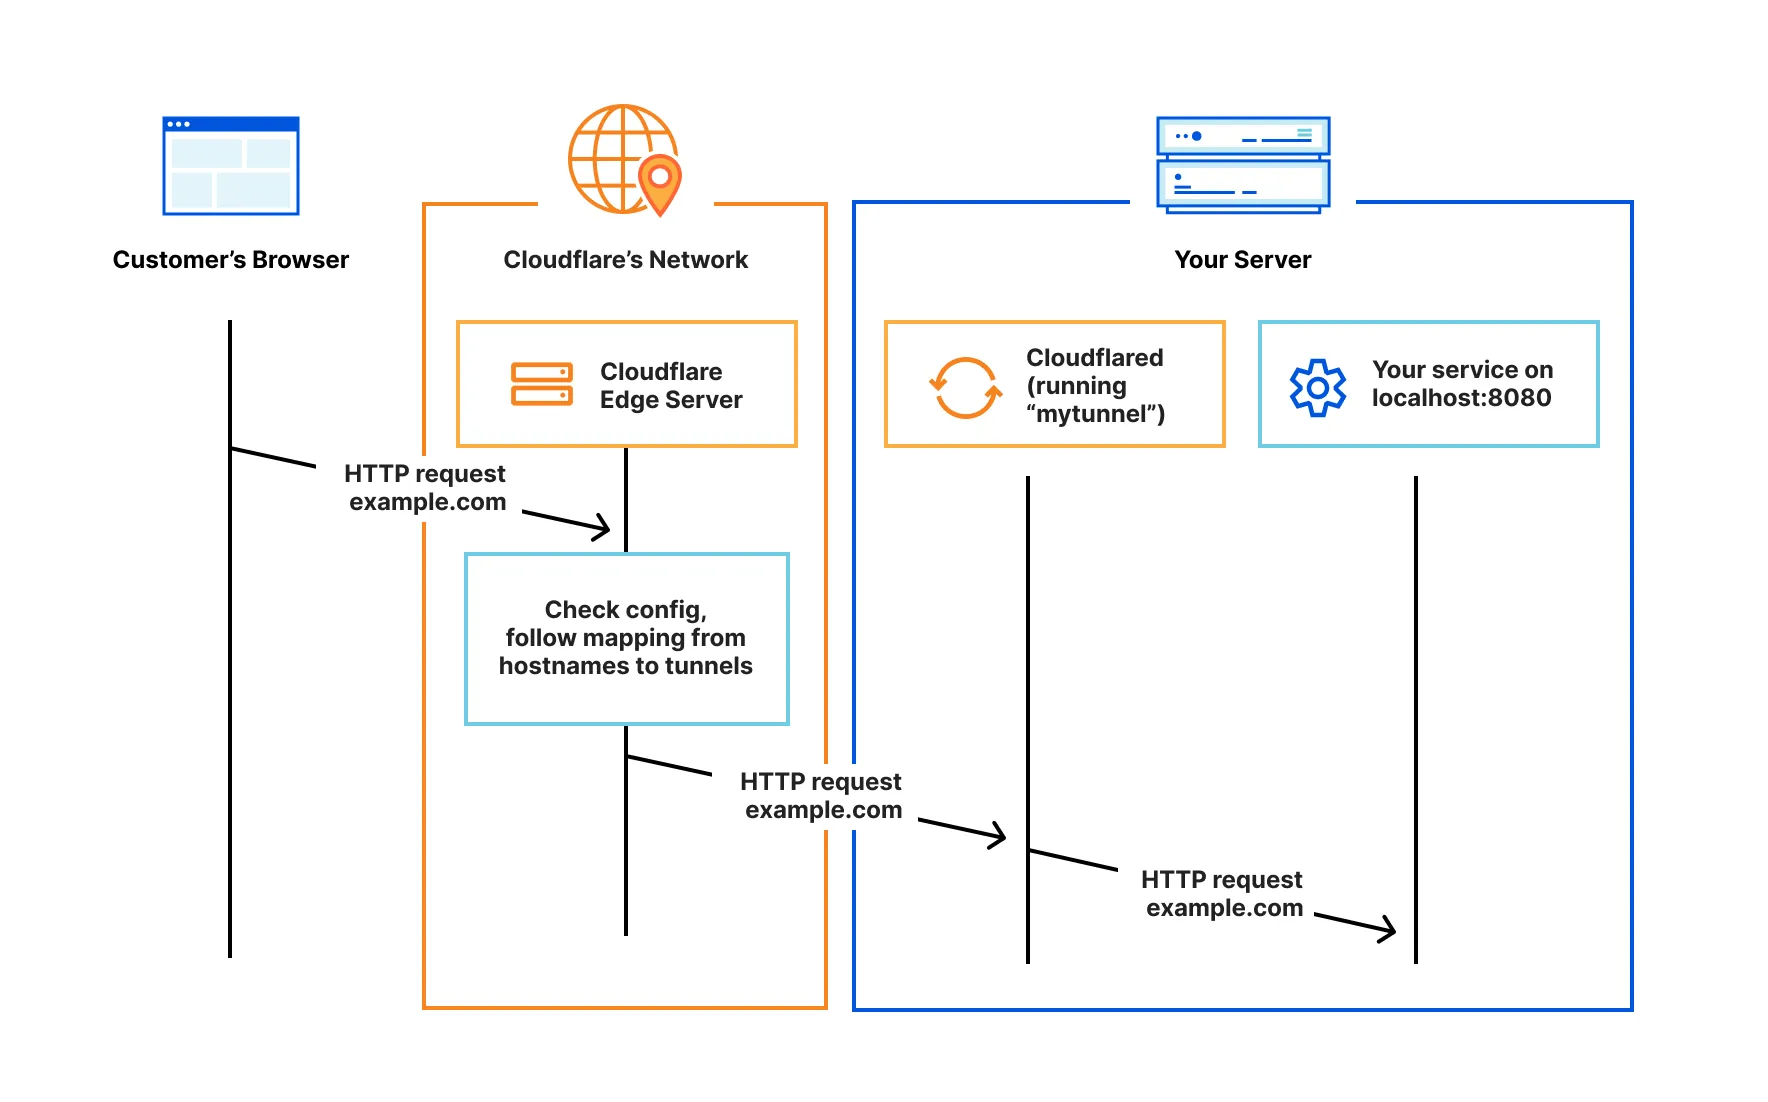
\includegraphics[width=1\textwidth]{imagenes/cloudflared.png}
  \caption{Esquema del funcionamiento de Cloudflare Tunnels \cite{cloudflaretunnels}.}
  \label{fig:cloudflared}
\end{figure}


\newpage
\section{Frontend}

%\subsection{Tecnologías}

El frontend está desarrollado utilizando Next.js 15 y TypeScript. Se aloja la web en Vercel por su extrema facilidad de uso, plan gratuito, auto-deploy desde GitHub, gran optimización y CDN global. La arquitectura se basa en componentes reutilizables y páginas especializadas que consumen la API del backend.



\subsection{Arquitectura de Componentes}

La estructura del frontend sigue las convenciones de Next.js con el nuevo App Router, organizando el código en:

\begin{itemize}
\item \textbf{Páginas:} Ubicadas en \texttt{src/app/}, incluyen la página principal, dashboard, búsqueda de pacientes, chat y visualizaciones específicas.
\item \textbf{Componentes:} En \texttt{src/components/}, contienen elementos reutilizables como el header, componentes de gráficos y elementos de UI.
\item \textbf{Hooks personalizados:} En \texttt{src/hooks/}, encapsulan lógica específica como el monitoreo de salud del backend.
\item \textbf{Tipos TypeScript:} En \texttt{src/types/}, definen las interfaces de datos para garantizar type safety.
\end{itemize}

Se utiliza Lucide React para iconografía consistente y Tailwind CSS para el diseño.

\subsection{Visualización de Datos}

Se ha implementado una estrategia progresiva para la visualización de datos, empleando dos librerías principales según la complejidad de cada caso. Para los gráficos más básicos se utiliza Observable Plot \cite{observableplot}, que ofrece soluciones preestablecidas y una integración sencilla. Cuando se requieren visualizaciones más complejas que demandan un control granular sobre el renderizado y la interactividad, se recurre a D3 \cite{d3}, también desarrollada por Observable, lo que permite adaptar los gráficos a necesidades avanzadas, sin salir del mismo ecosistema y estética.

Los componentes de visualización están diseñados como elementos autónomos que consumen datos de la API y manejan sus propios estados de carga y error. Esta aproximación facilita la reutilización y el testing individual de cada visualización.




\subsubsection{Tipos de visualización empleados}
En esta subsección se describen de forma teórica los tipos de gráficos utilizados, su propósito, cómo se interpretan y la librería empleada. No hace referencia a resultados específicos de la aplicación.

\paragraph{Population pyramid (Distribución por edad y género).} Muestra la distribución de una población por grupos de edad separada por género, permitiendo detectar envejecimiento, cohortes predominantes o asimetrías entre hombres y mujeres. Se interpreta leyendo barras horizontales a izquierda/derecha (generalmente hombres/mujeres) y el eje vertical con los grupos de edad. Implementado con Observable Plot \cite{populationPyramid,observableplot}.

\paragraph{Heatmap (Mapa de calor temporal).} Representa densidades o frecuencias mediante una cuadrícula coloreada. En contexto temporal, el eje X puede ser la hora o el día del mes y el eje Y el día de la semana o el mes; la intensidad de color codifica el número de eventos. Es útil para identificar patrones cíclicos o picos de actividad. Implementado con Observable Plot \cite{heatmap,observableplot}.

\paragraph{Horizontal bar chart (Barras horizontales).} Adecuado para comparar categorías con etiquetas largas. El eje Y contiene las categorías y el eje X el valor (p. ej., promedio de días). Facilita ordenar y comparar magnitudes. Implementado con Observable Plot \cite{hbarchart,observableplot}.

\paragraph{Sunburst (Jerarquía radial).} Visualiza jerarquías en anillos concéntricos; cada arco representa un nodo y su ángulo codifica el valor agregado. Permite hacer zoom para explorar niveles. Es útil para descomponer un total en categorías y subcategorías. Implementado con D3 \cite{sunburst,d3}.

\paragraph{Icicle (Jerarquía en segmentos).} Similar a sunburst pero en disposición rectangular; los rectángulos apilados muestran la jerarquía de mayor a menor nivel. El ancho representa el valor agregado. Adecuado para explorar taxonomías médicas y su contribución relativa. Implementado con D3 \cite{icicle,d3}.

\paragraph{Directed chord diagram (Flujos entre categorías).} Muestra flujos dirigidos entre nodos dispuestos en un círculo; el grosor del acorde codifica la intensidad del flujo y la dirección se indica con marcadores o asimetrías. Útil para analizar transferencias entre unidades o servicios. Implementado con D3 \cite{chord,d3}.

\subsection{Despliegue}

El frontend de la aplicación se ha desplegado públicamente utilizando la plataforma Vercel \cite{vercel}, una solución en la nube especializada en el despliegue de aplicaciones web modernas. 

Esta elección responde a varias ventajas clave para el proyecto. Por un lado, Vercel ofrece una integración nativa con Next.js, ya que es la empresa creadora de este framework. Esto permite contar con soporte optimizado y características específicas, como la optimización automática de bundles, el Server-Side Rendering (SSR) y la Static Site Generation (SSG). Además, la plataforma distribuye la aplicación a través de su red global de servidores edge, lo que garantiza tiempos de carga mínimos desde cualquier ubicación geográfica. Otro aspecto relevante es la rapidez en los despliegues, que suelen completarse en menos de 30 segundos y facilitan iteraciones ágiles durante el desarrollo. Finalmente, Vercel dispone de un plan gratuito generoso, ideal para entornos académicos y de desarrollo, que incluye 100GB de ancho de banda mensual, despliegues ilimitados y la posibilidad de utilizar un dominio personalizado.

El proceso de despliegue se gestiona de manera automática gracias a la integración por defecto entre Vercel y GitHub. Al importar el repositorio del proyecto Next.js, Vercel configura automáticamente un flujo de integración y entrega continua (CI/CD), sin necesidad de implementarlo manualmente. De este modo, cada vez que se realiza un push al repositorio principal, Vercel detecta los cambios y ejecuta los comandos de construcción de Next.js (\texttt{npm run build}), optimizando el código para producción. Durante este proceso, también se realizan las validaciones de TypeScript y ESLint configuradas en el proyecto. Una vez completada la construcción, la nueva versión se despliega de forma atómica, garantizando que no exista tiempo de inactividad, y se invalida automáticamente la caché de la CDN para asegurar que los usuarios reciban de inmediato la versión actualizada.

Gracias a este sistema, la versión en producción refleja siempre el estado más reciente del código en el repositorio principal, lo que facilita la colaboración en el desarrollo y reduce significativamente el riesgo de errores humanos durante el despliegue. La aplicación frontend está accesible en producción a través de la URL \url{https://tfg.angeloyo.com}.


\begin{figure}[H]
  \centering
  \fbox{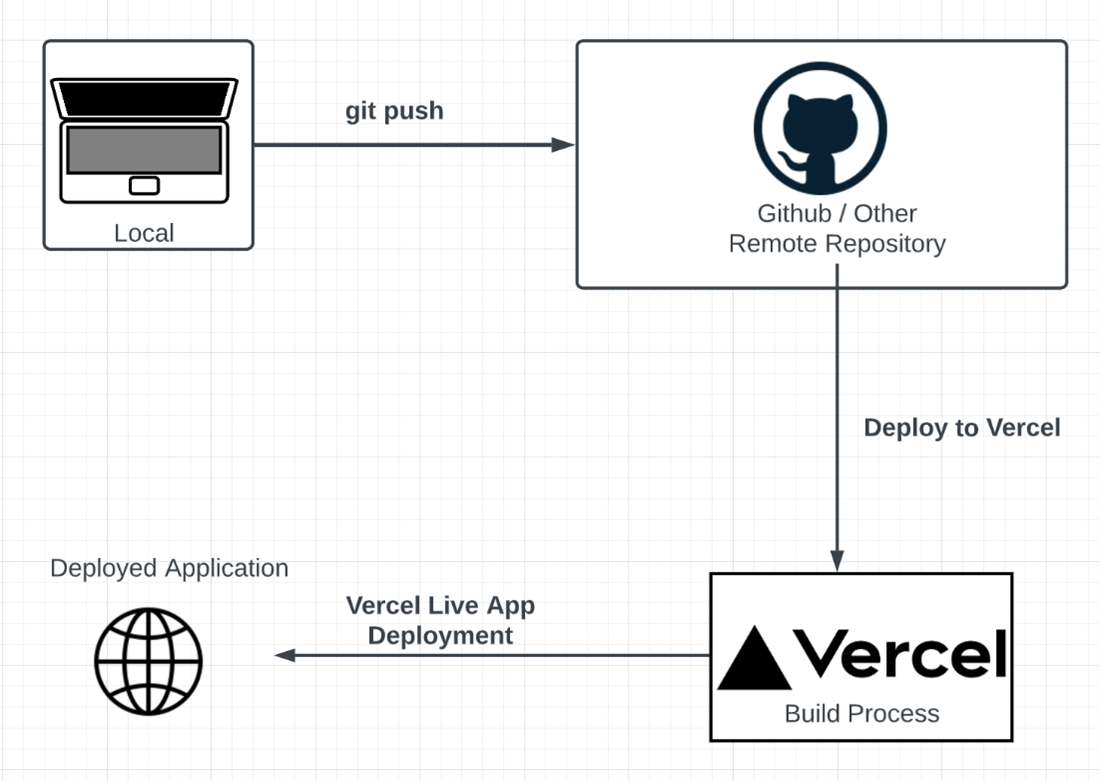
\includegraphics[width=0.8\textwidth]{imagenes/cicd.png}}
  %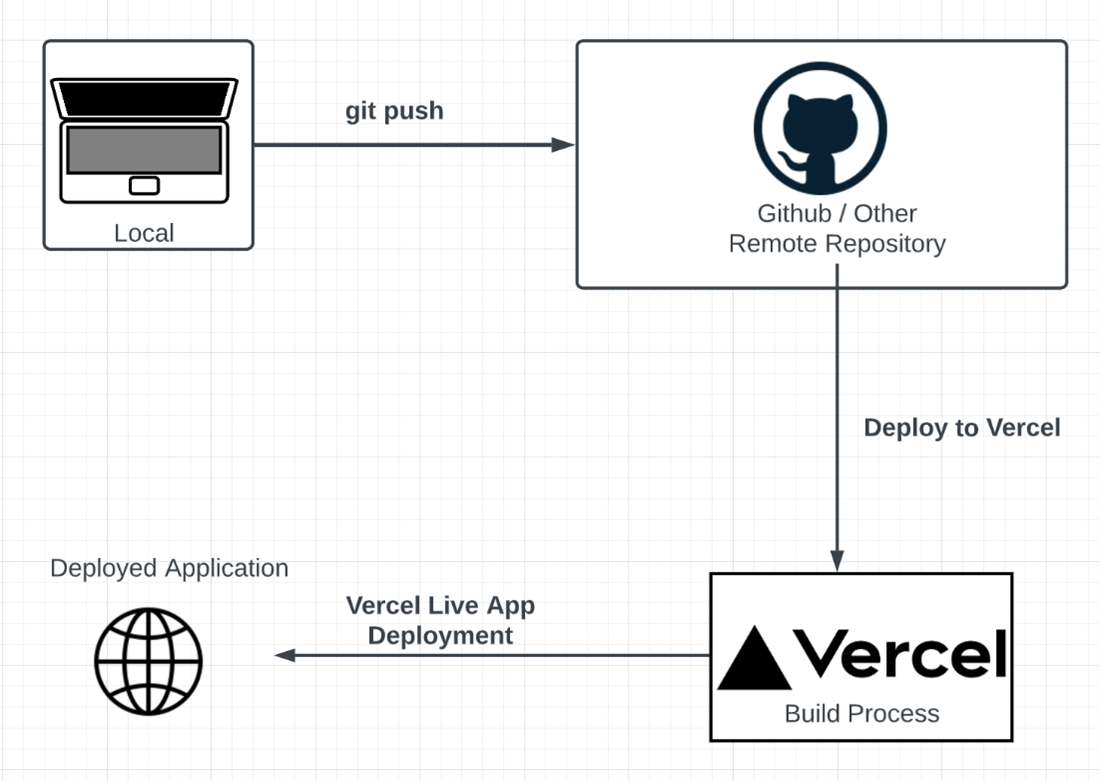
\includegraphics[width=0.8\textwidth]{imagenes/cicd.png}
  \caption{Esquema del depliegue con Vercel \cite{cicdfoto}.}
  \label{fig:cicd}
\end{figure}
